\documentclass[12pt]{article}

\usepackage[T2A]{fontenc}
\usepackage[utf8]{inputenc}
\usepackage[russian]{babel}
\usepackage{amsthm, amsmath, amssymb,amsfonts}
\usepackage{hologo}
\usepackage{graphicx}
\usepackage{lipsum}

% Настройка полей документа
\usepackage[top=2cm, bottom=2cm, left=2cm, right=2cm]{geometry}

\usepackage{booktabs}
\usepackage{multirow}
\usepackage[table]{xcolor}
\usepackage{array}
\usepackage{colortbl}

\usepackage{listings}
\usepackage{xcolor}
\usepackage{amsfonts}

\newcounter{mysectioncounter}
\newcommand{\mysection}[1]{
  \vspace{0.5em}
  \refstepcounter{mysectioncounter}
  {\large\bf \arabic{mysectioncounter}. #1} 
  \vspace{0.5em}
}

\newcommand{\RomanNumeralCaps}[1]{\MakeUppercase{\romannumeral #1}}

\begin{document}

\section{Описание кода}

\subsection{Договор про хранение графов}
\textbf{Граф хранится в специальном классе со следующими полями:}

\begin{itemize}
    \item Вершины графа хранятся списком:
    \[ V_G = (x_1, x_2, \ldots, x_k) \]
    где $k$ - количество вершин графа, $x_i$ - координата $i$-ой вершины
    
    \item Рёбра графа хранятся множеством:
    \[ E_G = \{(a_1, b_1), (a_2, b_2), \ldots\} \]
    где $a_i < b_i$ - номера вершин
    
    \item Также хранится объект \texttt{NetworkX.Graph} для удобного использования различных алгоритмов на графах
\end{itemize}

\textbf{Класс имеет 3 метода:}
\begin{enumerate}
    \item Два метода для построения рёбер, соответствующих:
    \begin{itemize}
        \item KNN-графу
        \item Distance-графу
    \end{itemize}
    \item Один метод для визуализации графа
\end{enumerate}


\textbf{Ниже приведена UML-диграмма класса}\\
\begin{center}
    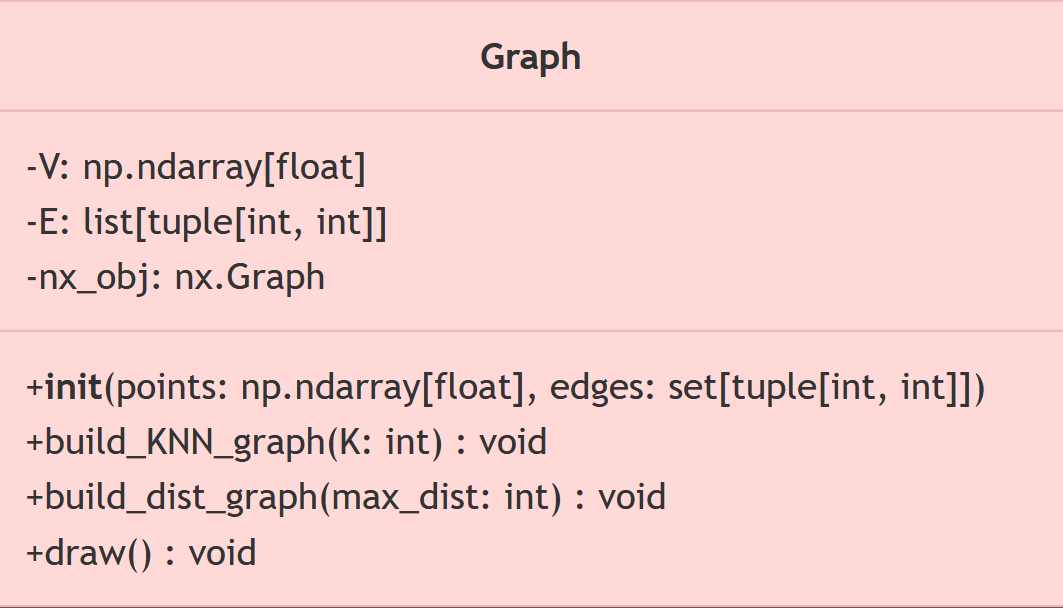
\includegraphics[width=0.6\textwidth]{graphs_implementation/UML graph.png}\\    
\end{center}


    
\subsection{Функции подсчета характеристик графа}
\input code-format.tex

В данном разделе представлены ключевые функции для анализа свойств графов. Все функции принимают на вход объект класса \texttt{Graph} и возвращают числовые характеристики.

\begin{lstlisting}
def calculate_min_deg(G: Graph) -> int:
    """ Returns the minimum degree of a graph vertex """

def calculate_max_deg(G: Graph) -> int:
    """ Returns the maximum degree of a graph vertex """

def calculate_number_component(G: Graph) -> int:
    """ Returns the number of connected components of a graph """

def calculate_number_articul(G: Graph) -> int:
    """ Returns the number of articulation points of a graph """

def calculate_number_triangle(G: Graph) -> int:
    """ Returns the number of triangles in a graph """

def calculate_clique_number(G: Graph) -> int:
    """ Returns the click count of a graph """

def calculate_maxsize_independed_set(G: Graph) -> int:
    """ Returns the size of the maximum independent set """
\end{lstlisting}

\noindent Все функции реализованы с помощью библиотеки \textbf{NetworkX}. Почти все функции честным перебором дают точные значения характеристик.\\
Исключениями являются:

\begin{itemize}
    \item Функция подсчета кликового числа. Реализована через жадный поиск хроматического числа графа, основано на том, что для дистанционного графа они совпадают почти наверное.

    \item Функция подсчета числа независимости графа. Реализована через подсчет кликового числа для дополнения.
\end{itemize}

\noindentКаждая функция покрыта тестами.

\newpage
\section*{2. Part-I}

\subsection*{2.1 Поведение характеристики в зависимости от параметров распределений (Минаков Д.Д)}

Выберем 3 модели - линейная, логистическая и ridge регрессии, обучим на них классификатор и сравним качество

\begin{table}[h]
    \centering
    \label{tab:results}
    \begin{tabular}{cccccc}
    \toprule
    N & Модель & Precision & Accuracy & Recall \\
    \midrule
    \multirow{3}{*}{25} 
        & Logistic & 0.8071 & 0.8037 & 0.7980 \\
        & Linear & 0.8426 & 0.8077 & 0.7567 \\
        & Ridge & 0.8426 & 0.8077 & 0.7567 \\
    \hline
    \multirow{3}{*}{100} 
        & Logistic & 0.9700 & 0.9693 & 0.9687 \\
        & Linear & 0.9907 & 0.9597 & 0.9280 \\
        & Ridge & 0.9907 & 0.9597 & 0.9280 \\
    \hline
    \multirow{3}{*}{500} 
        & Logistic & 1.0000 & 0.9993 & 0.9987 \\
        & Linear & 1.0000 & 0.9993 & 0.9987 \\
        & Ridge & 1.0000 & 0.9993 & 0.9987 \\
    \bottomrule
    \end{tabular}
\end{table}

Все линейные модели дают очень близкий результат, поэтому зафиксируем в качестве модели обычную \textbf{логистическую регрессию}\\

\textbf{Проведем кроссвалидацию для оценки дисперсии метрик}\\

\hspace*{-1cm}
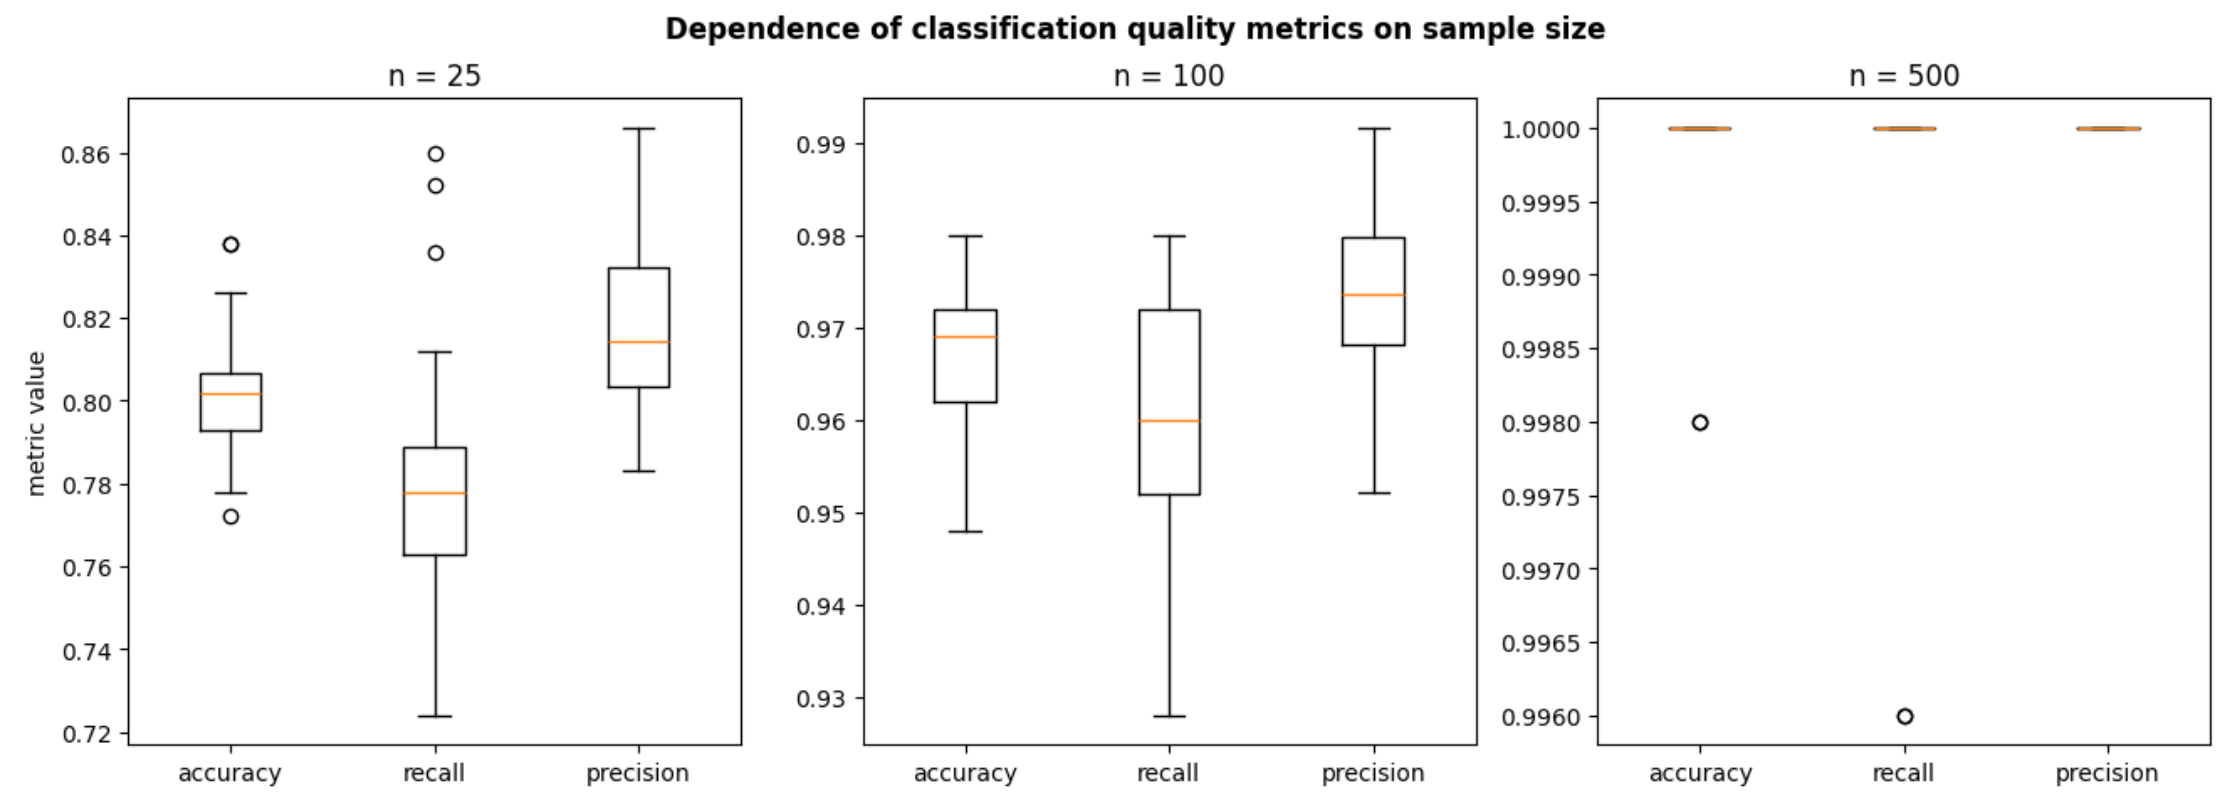
\includegraphics[width=1\textwidth]{Part-II_student-2/dependence metrics on sample size}\\ 

\textbf{Занесем данные в таблицу}\\

\begin{table}[h]
    \centering
    \begin{tabular}{lccc}
    \toprule
    \textbf{Размер выборки} & \textbf{Метрика} & \textbf{Среднее} & \textbf{Дисперсия} \\
    \midrule
    \multirow{3}{*}{N=25} 
     & Accuracy  & 0.80  & 0.000271 \\
     & Recall    & 0.78  & 0.001231 \\
     & Precision & 0.81  & 0.000460 \\
    \midrule
    \multirow{3}{*}{N=100}
     & Accuracy  & 0.97  & $6.384 \times 10^{-5}$ \\
     & Recall    & 0.96  & 0.000166 \\
     & Precision & 0.97  & $9.624 \times 10^{-5}$ \\
    \midrule
    \multirow{3}{*}{N=500}
     & Accuracy  & 0.999 & $3.6 \times 10^{-7}$ \\
     & Recall    & 0.999 & $1.44 \times 10^{-6}$ \\
     & Precision & 0.99  & 0.0 \\
    \bottomrule
    \end{tabular}
\end{table}

\noindent\textbf{Выводы:}
\begin{itemize}
    \item Увеличение выборки снижает дисперсию экспоненциально

    \item \textbf{Стабильность метрик:}
        \begin{itemize}
            \item Precision демонстрирует самую низкую дисперсию на всех выборках
            \item Recall наиболее чувствителен к размеру выборки

        \end{itemize}
    
    \item \textbf{Оптимальный размер:} Для данной задачи выборка размером n=100 уже обеспечивает отличные результаты, а дальнейшее увеличение (n=500) лишь незначительно улучшает метрики и их стабильность.
\end{itemize}

\restoregeometry
\newpage

\subsection*{2.1 Поведение характеристики в зависимости от параметров распределений (Иванова А.А)}
Посмотрим на поведение характеристик при фиксированных параметрах построения графов для распределения Лапласа и косого нормального, с варьирующимися параметрами распределений. Ниже графики, на которых перебираются различные параметры $\alpha_{laplace}, \beta_{laplace}, \alpha_{skew}$ при фиксированных параметрах графа:
\begin{itemize}
    \item Размер графа =  40
    \item K в KNN = 3
    \item dist в Distance = 1
    \item характеристика для KNN графа - число треугольников (на этой странице)
    \item характеристика для Dist графа - максимальное независимое множество
\end{itemize}
\\

\hspace*{-1cm}
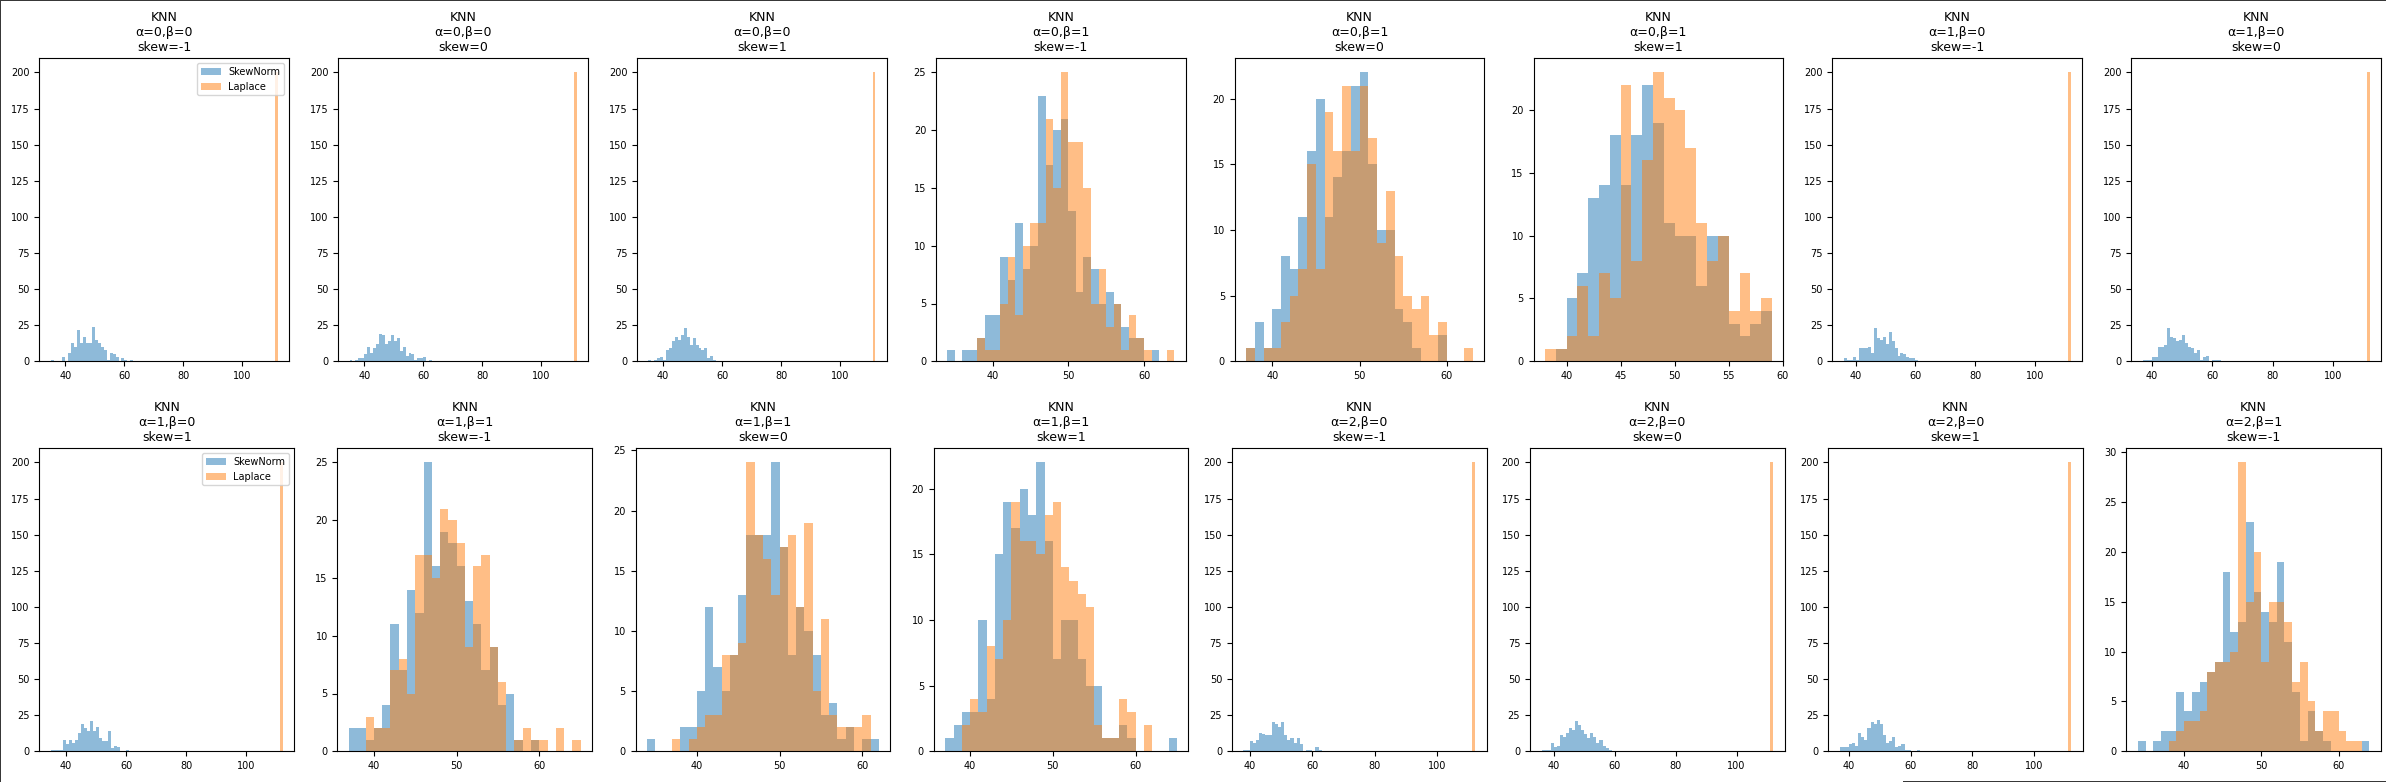
\includegraphics[width=1\textwidth]{Part-I-Ivanova/1_hist.png}\\ 
\hspace*{-0.5cm}
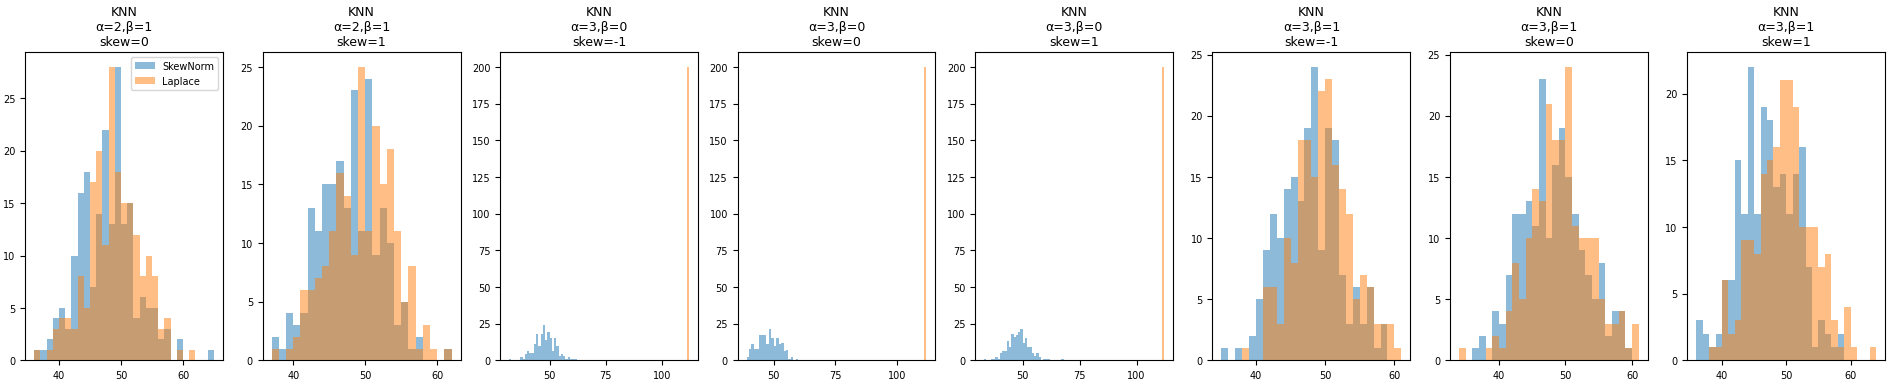
\includegraphics[width=1\textwidth]{Part-I-Ivanova/4_hist.png}\\ 
\textbf{Вывод:} в зависимости от параметров распределений характеристика 'Количество треугольников' KNN графа может быть \textbf{очень хорошим} признаком классификации при хороших параметрах распределений, а при некоторых графики практически идентичны, распределения трудно отличимы.
\newpage
\noindent\textbf{Далее графики для дистанционного графа :} \\\\


\hspace*{-1cm}
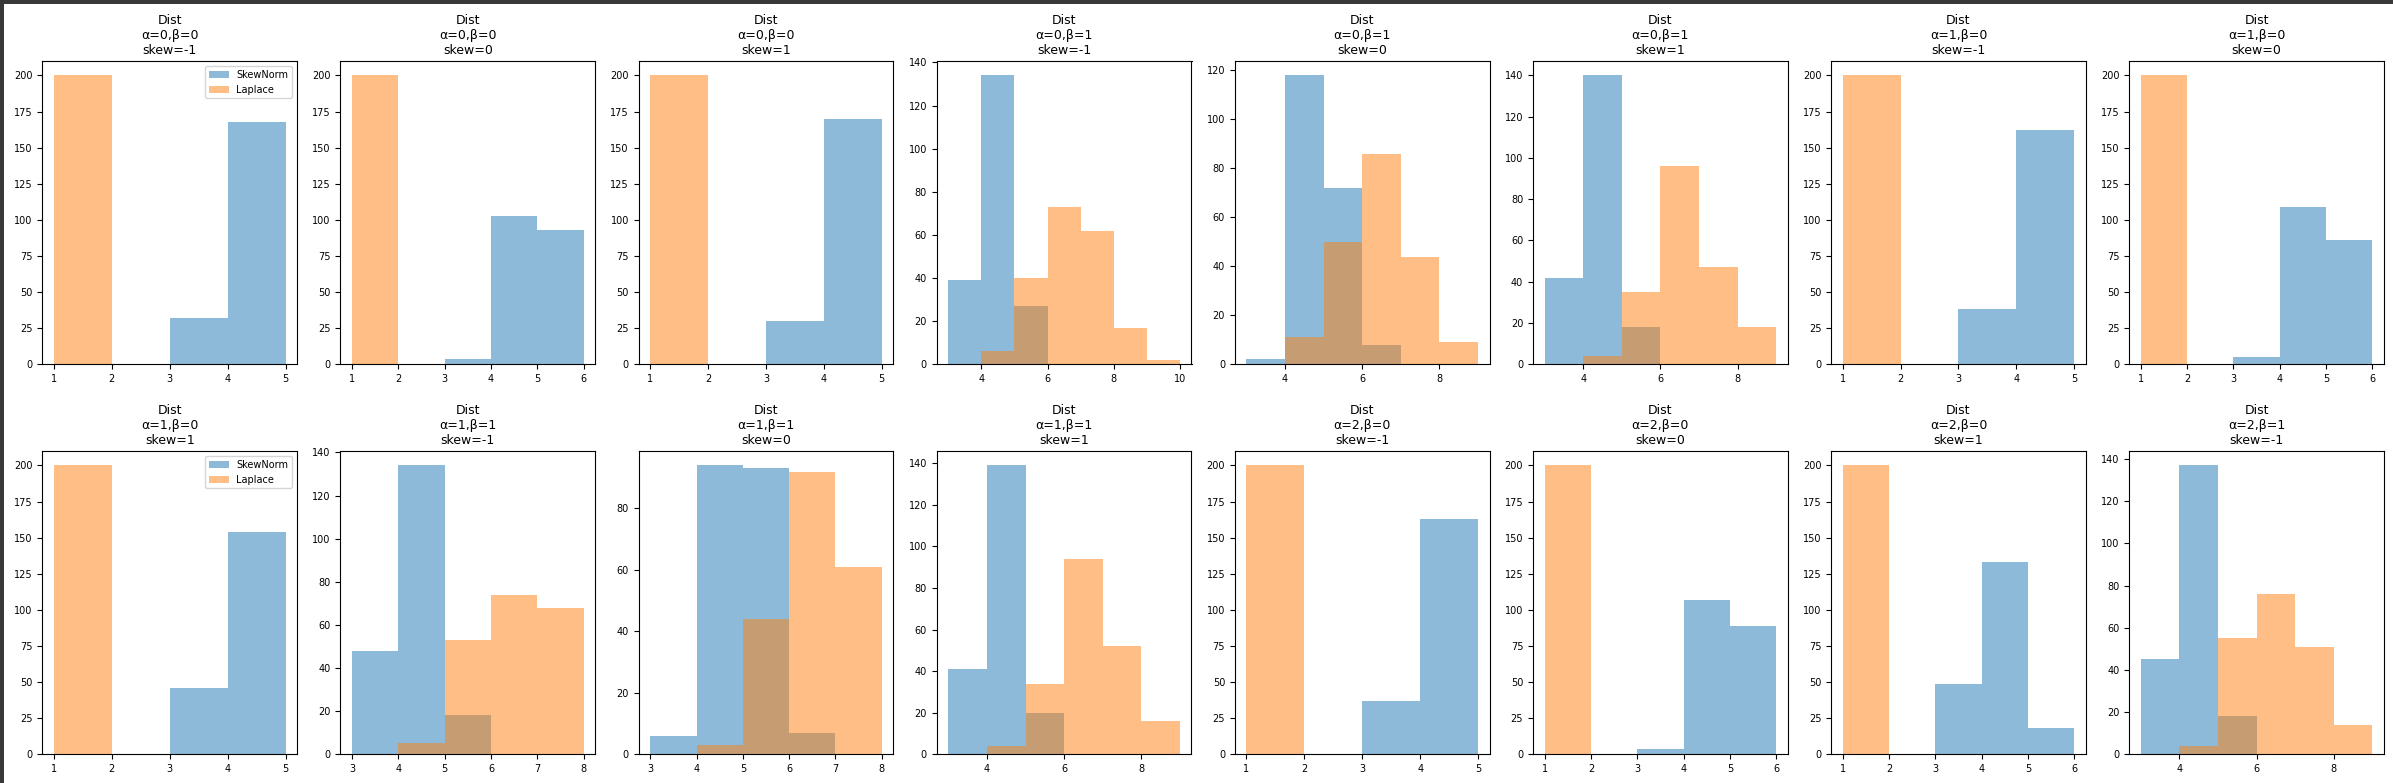
\includegraphics[width=1\textwidth]{Part-I-Ivanova/2_hist.png}
\\
\hspace*{-0.5cm}
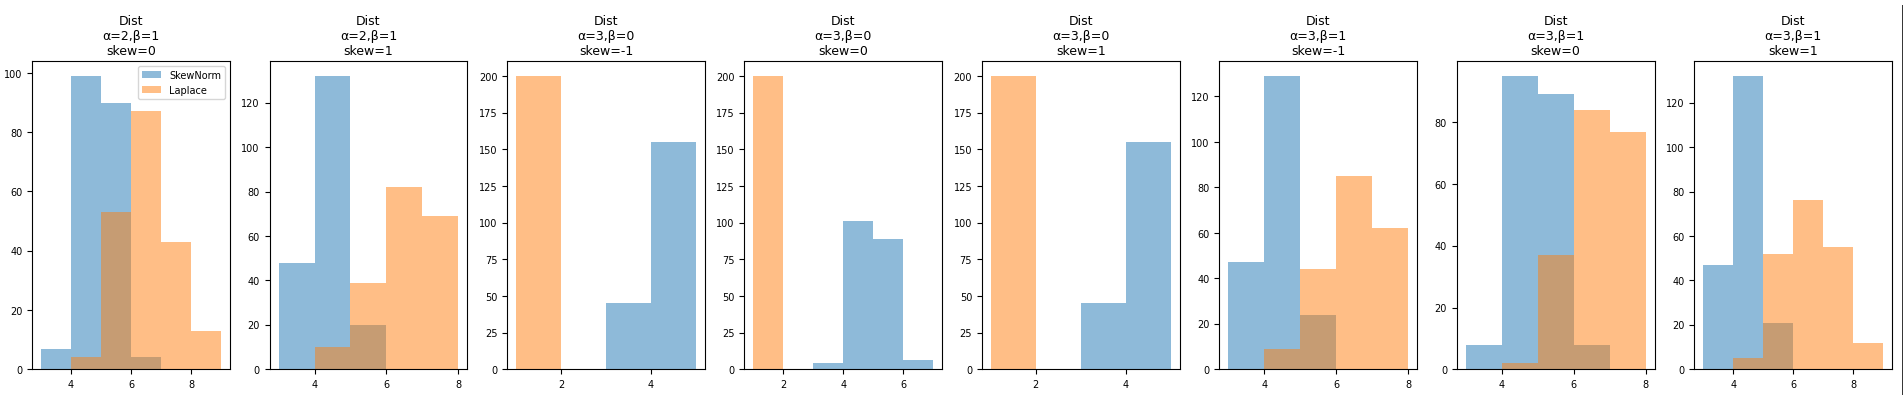
\includegraphics[width=1\textwidth]{Part-I-Ivanova/3_hist.png}\\ 


\noindent\textbf{Вывод:} в целом характеристика 'Размер максимального независимого множества' неплохая характеристика, при некоторых параметрах она лучше разделяет распределения, в некоторых хуже, но в целом всегда неплохо.

\newpage

\subsection*{2.2 Поведение характеристики в зависимости от построения\\ (Минаков Д.Д.)}

Теперь посмотрим на поведение характеристик в зависимости от параметров построения графов, при фиксированных распределениях
\begin{equation*}
    \text{Weibull}(\ \frac{1}{2}, \frac{1}{\sqrt{10}}) \qquad\qquad \Gamma(\ \frac{1}{2}, \frac{1}{\sqrt2})
\end{equation*}

\hspace*{-1cm}
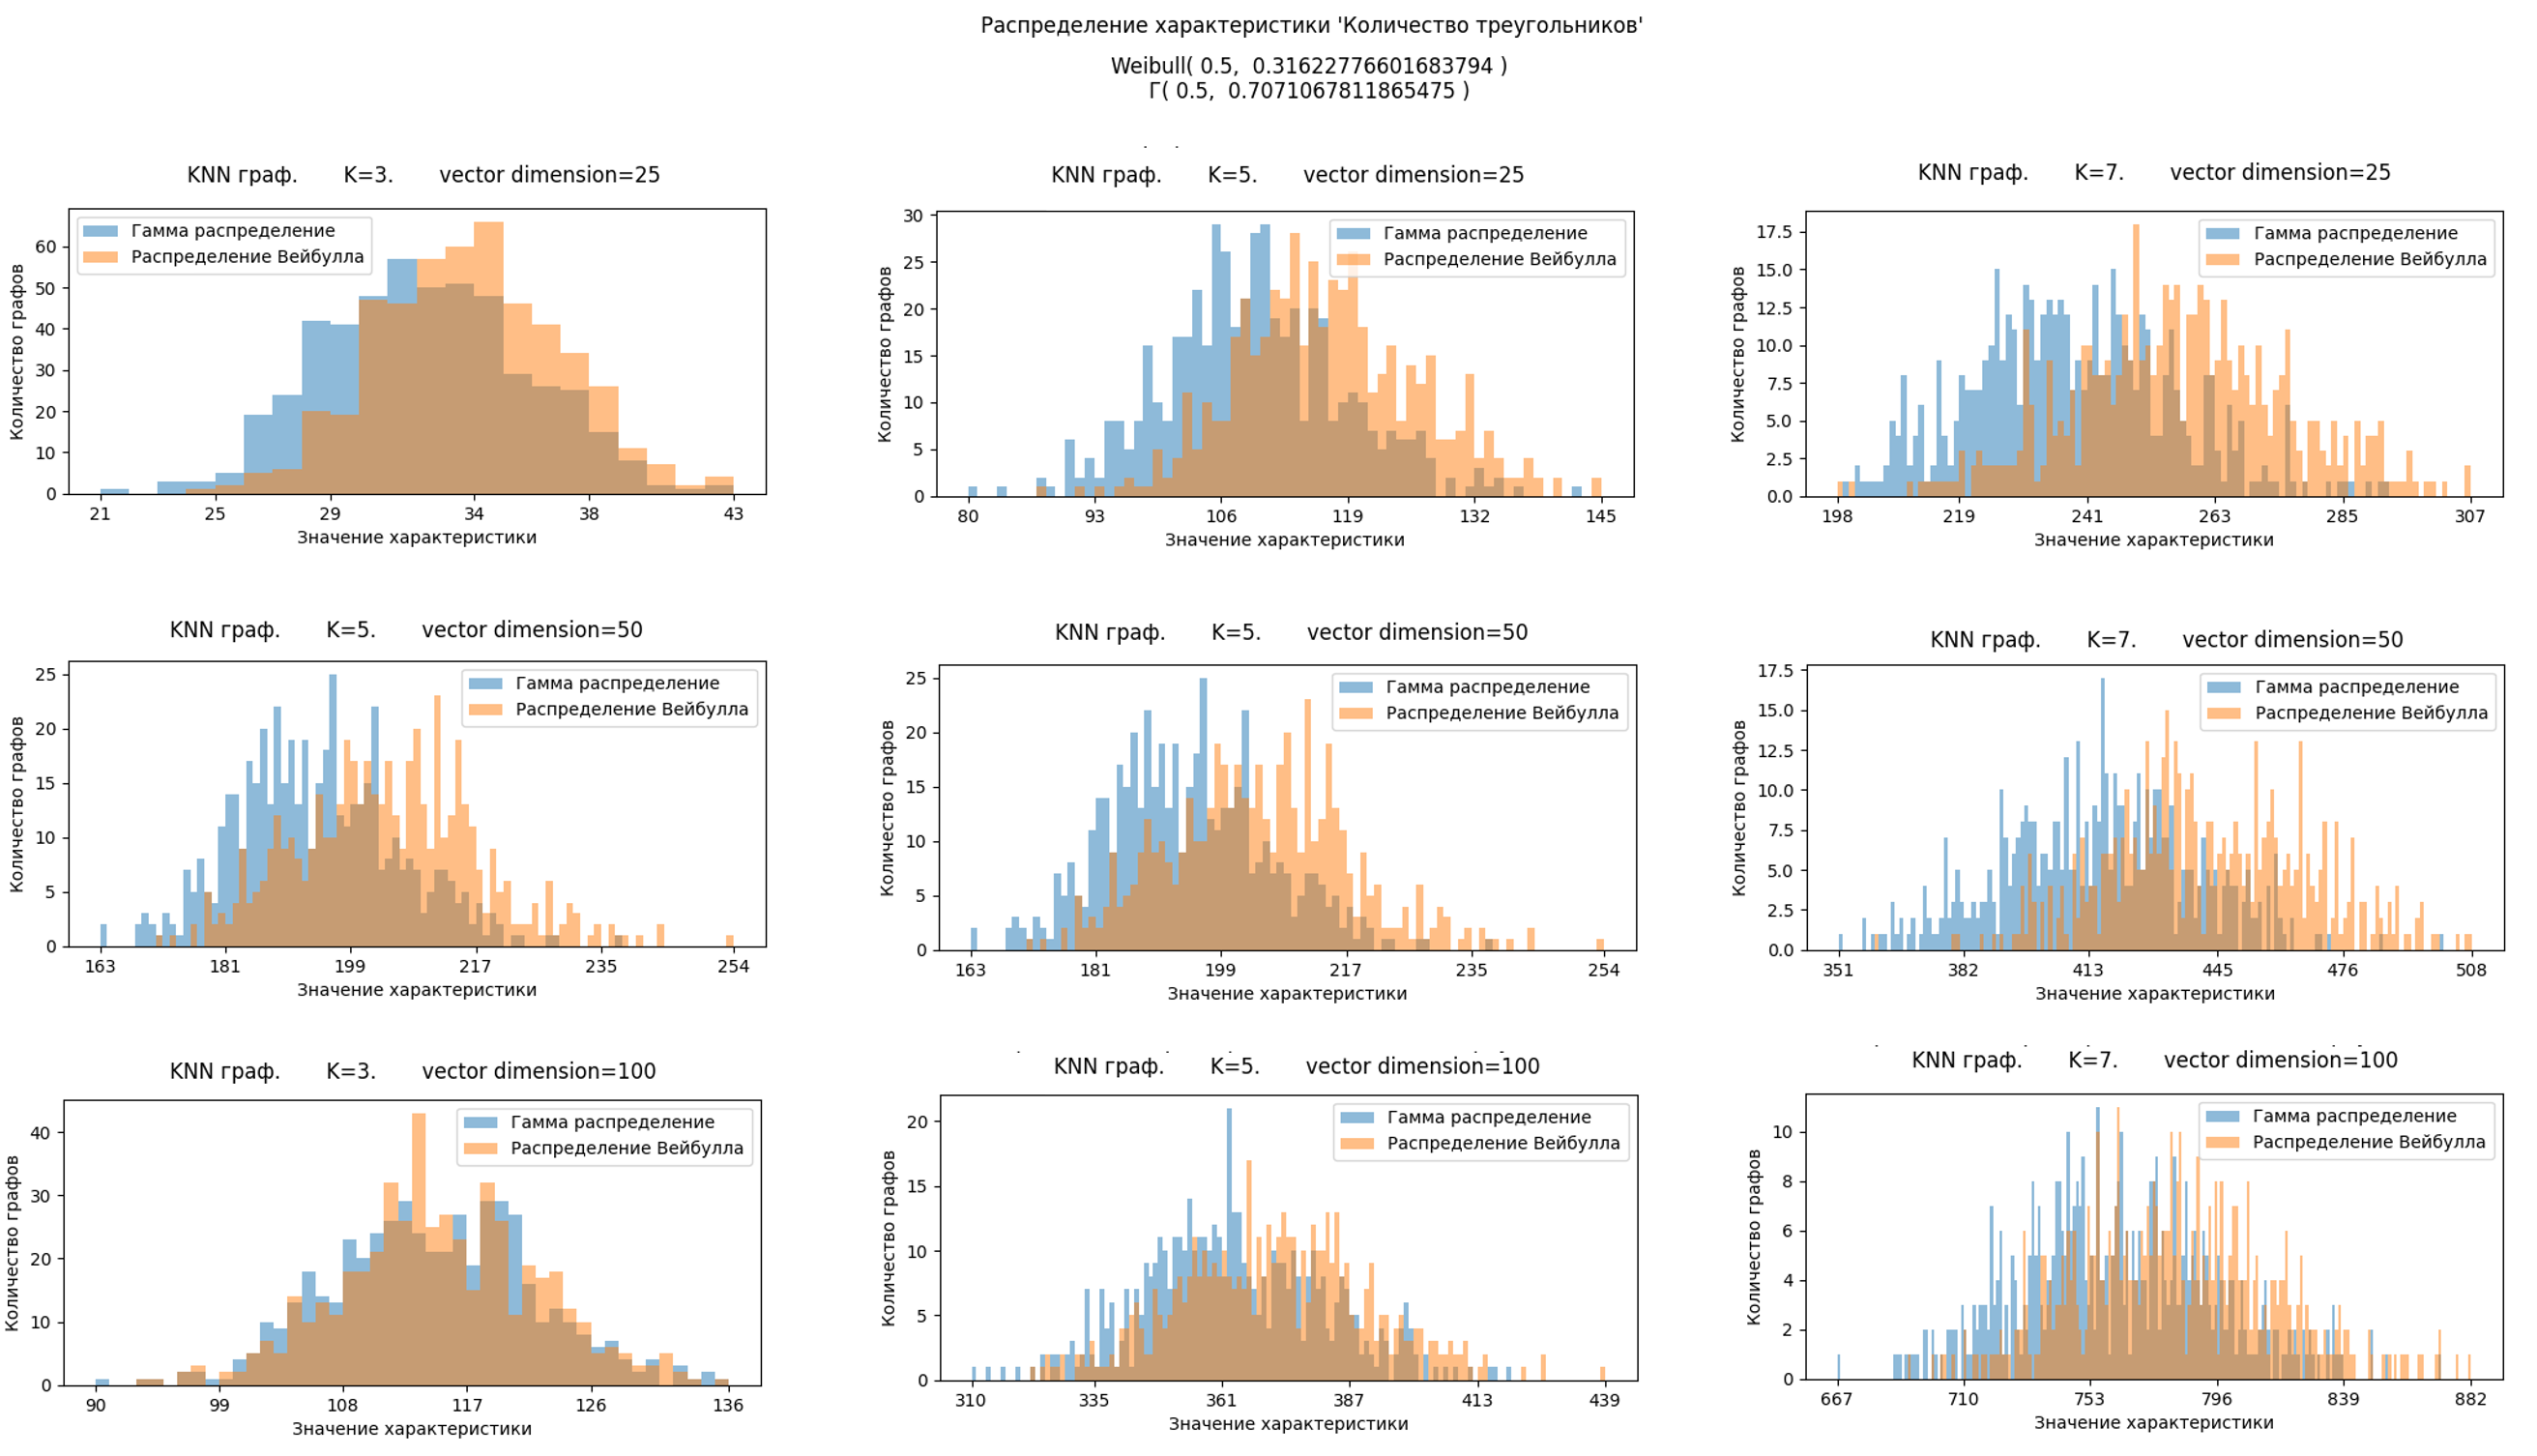
\includegraphics[width=1\textwidth]{Part-I_student-2/point 2_histogram_KNN.png}\\ 

\textbf{Вывод:} при большом размере выборки, количество треугольников выглядит как не самая удачная характеристика для классификации, однако, при относительно небольшой выборке ($\leq 50$), эта характеристика может оказаться неплохим второстепенным признаком.\\ 

\hspace*{-1cm}
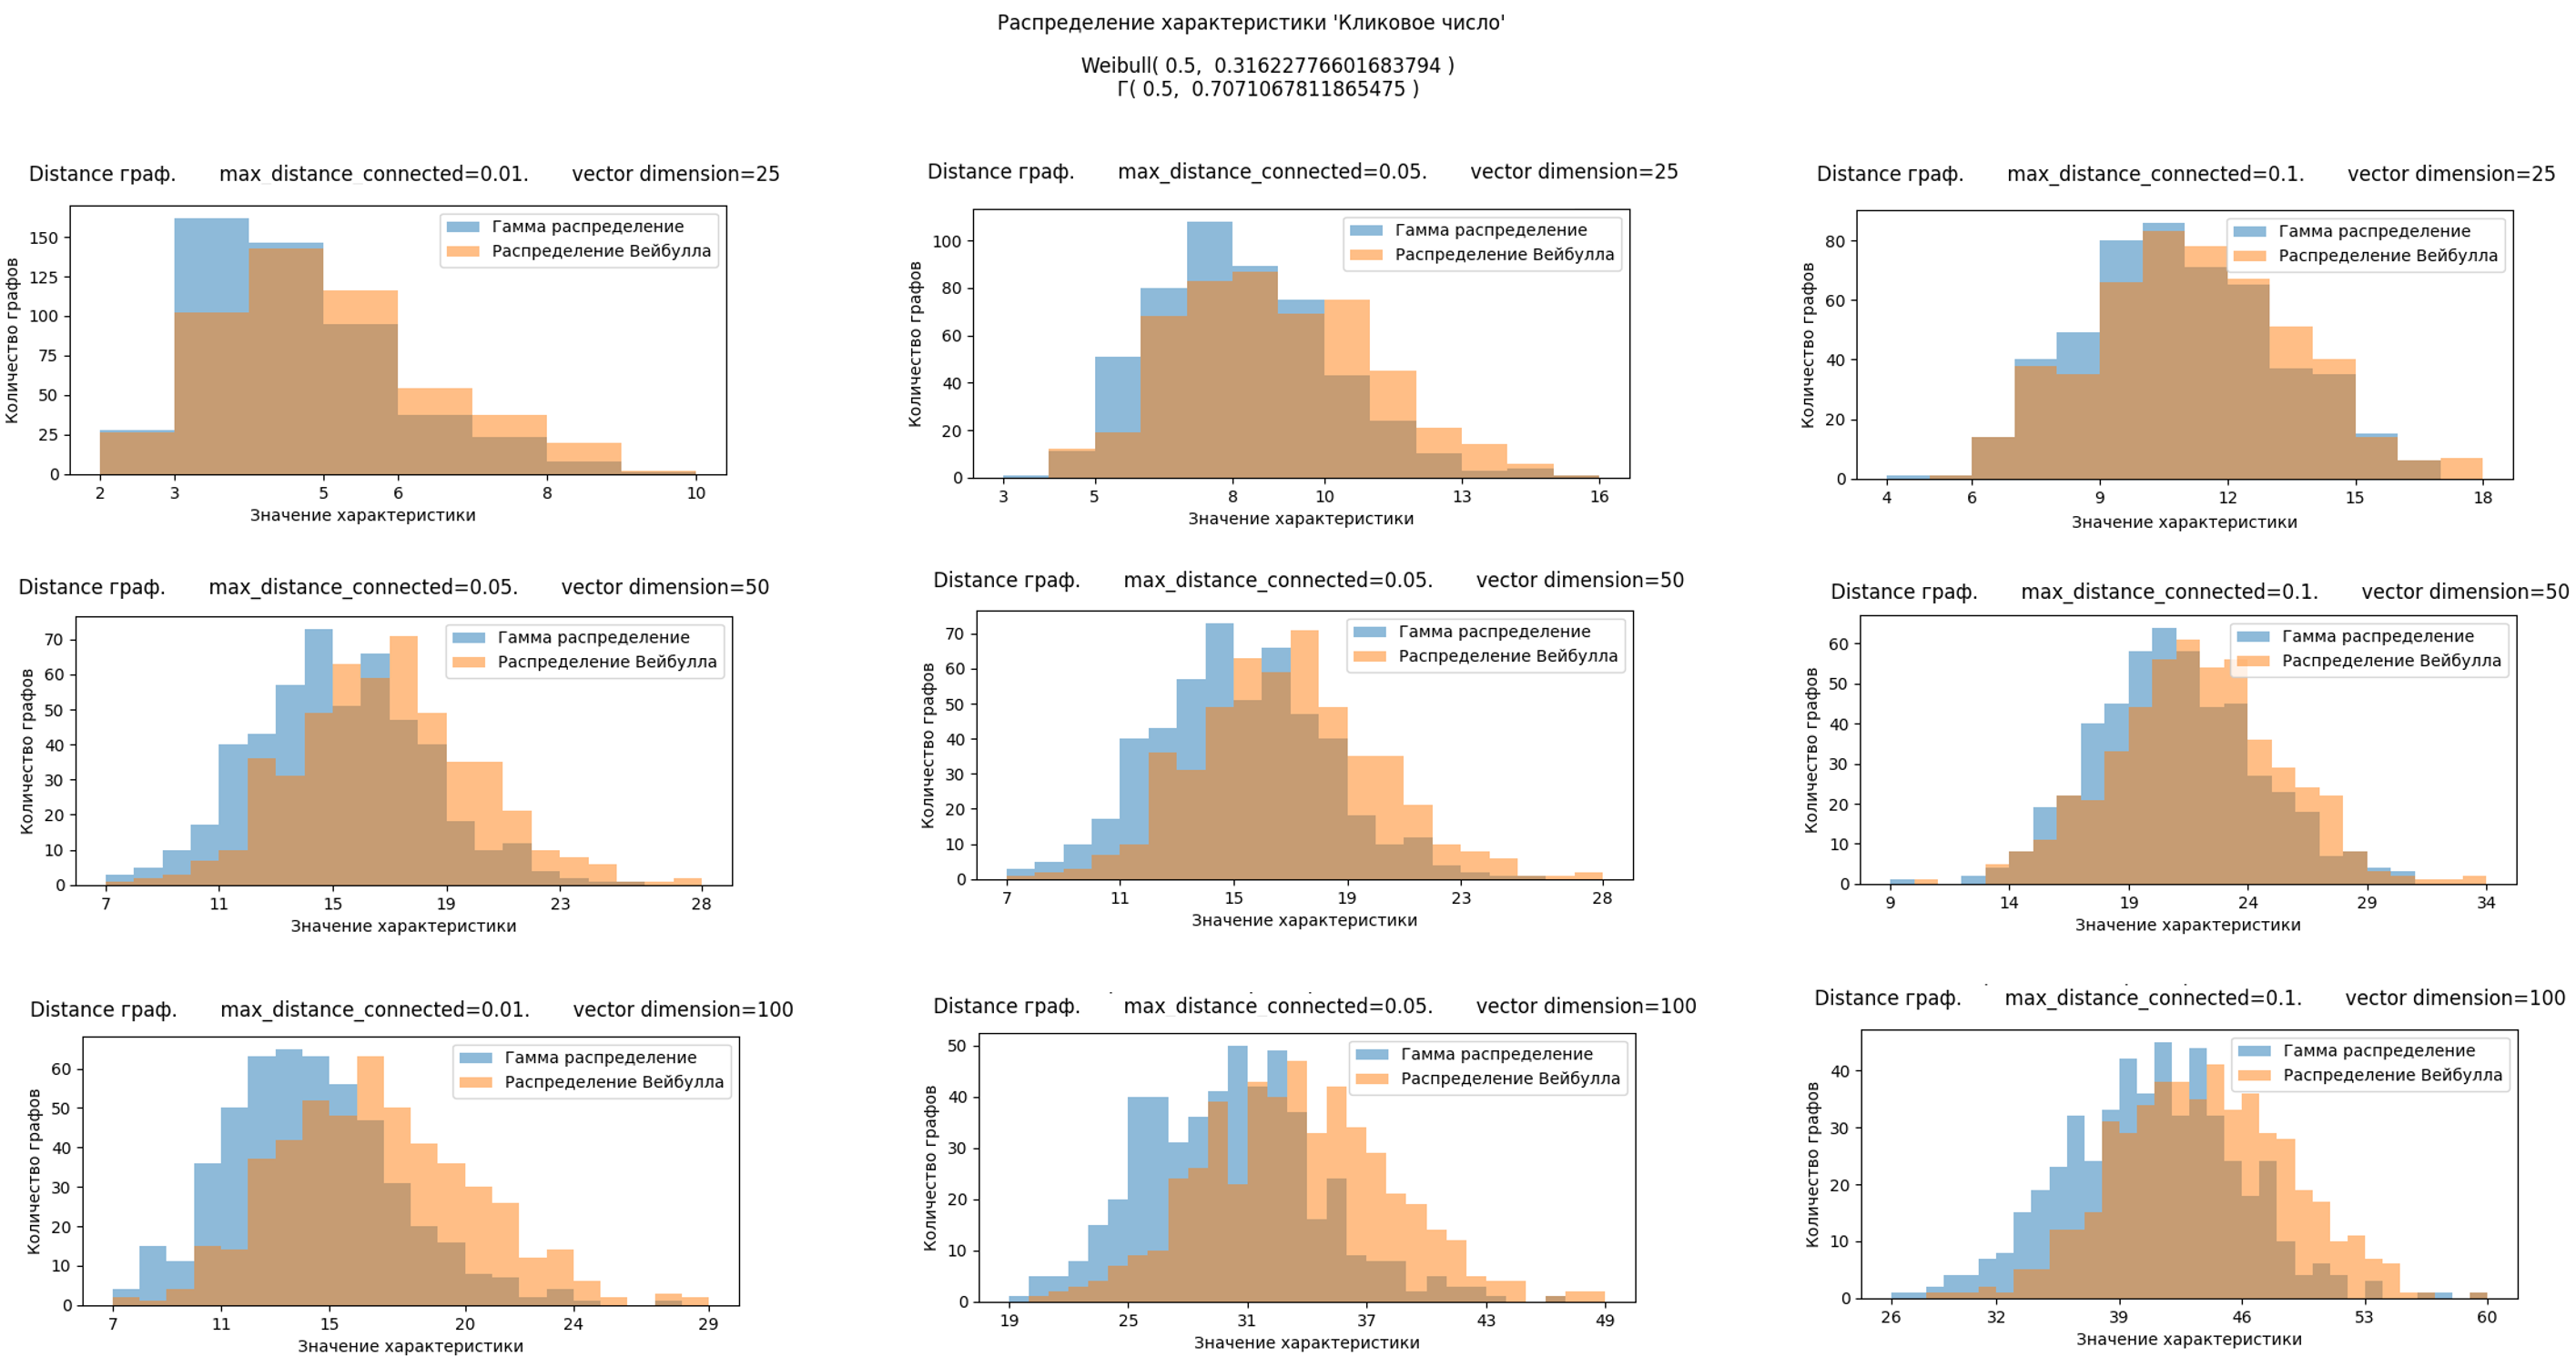
\includegraphics[width=1\textwidth]{Part-I_student-2/point 2_histogram_Dist.png}\\ 

\textbf{Вывод:} кликовое число, с точки зрения задачи классификации, для данных распределений является посредственным признаком, независимо от размера выборки и расстояния связи. Убедиться в этом  еще раз мы сможем в \textbf{Part-II}. 
\newpage

\subsection*{2.2 Поведение характеристики в зависимости от построения \\(Иванова А.А.)}

Теперь посмотрим на поведение характеристик в зависимости от параметров построения графов, при фиксированных распределениях
\\
\begin{equation*}
    \text{Laplace}(\ 0, \frac{1}{\sqrt{2}}) \qquad\qquad Skewnormal (1)
\end{equation*}
\textbf{Графики для KNN графа :}


\hspace*{-1cm}
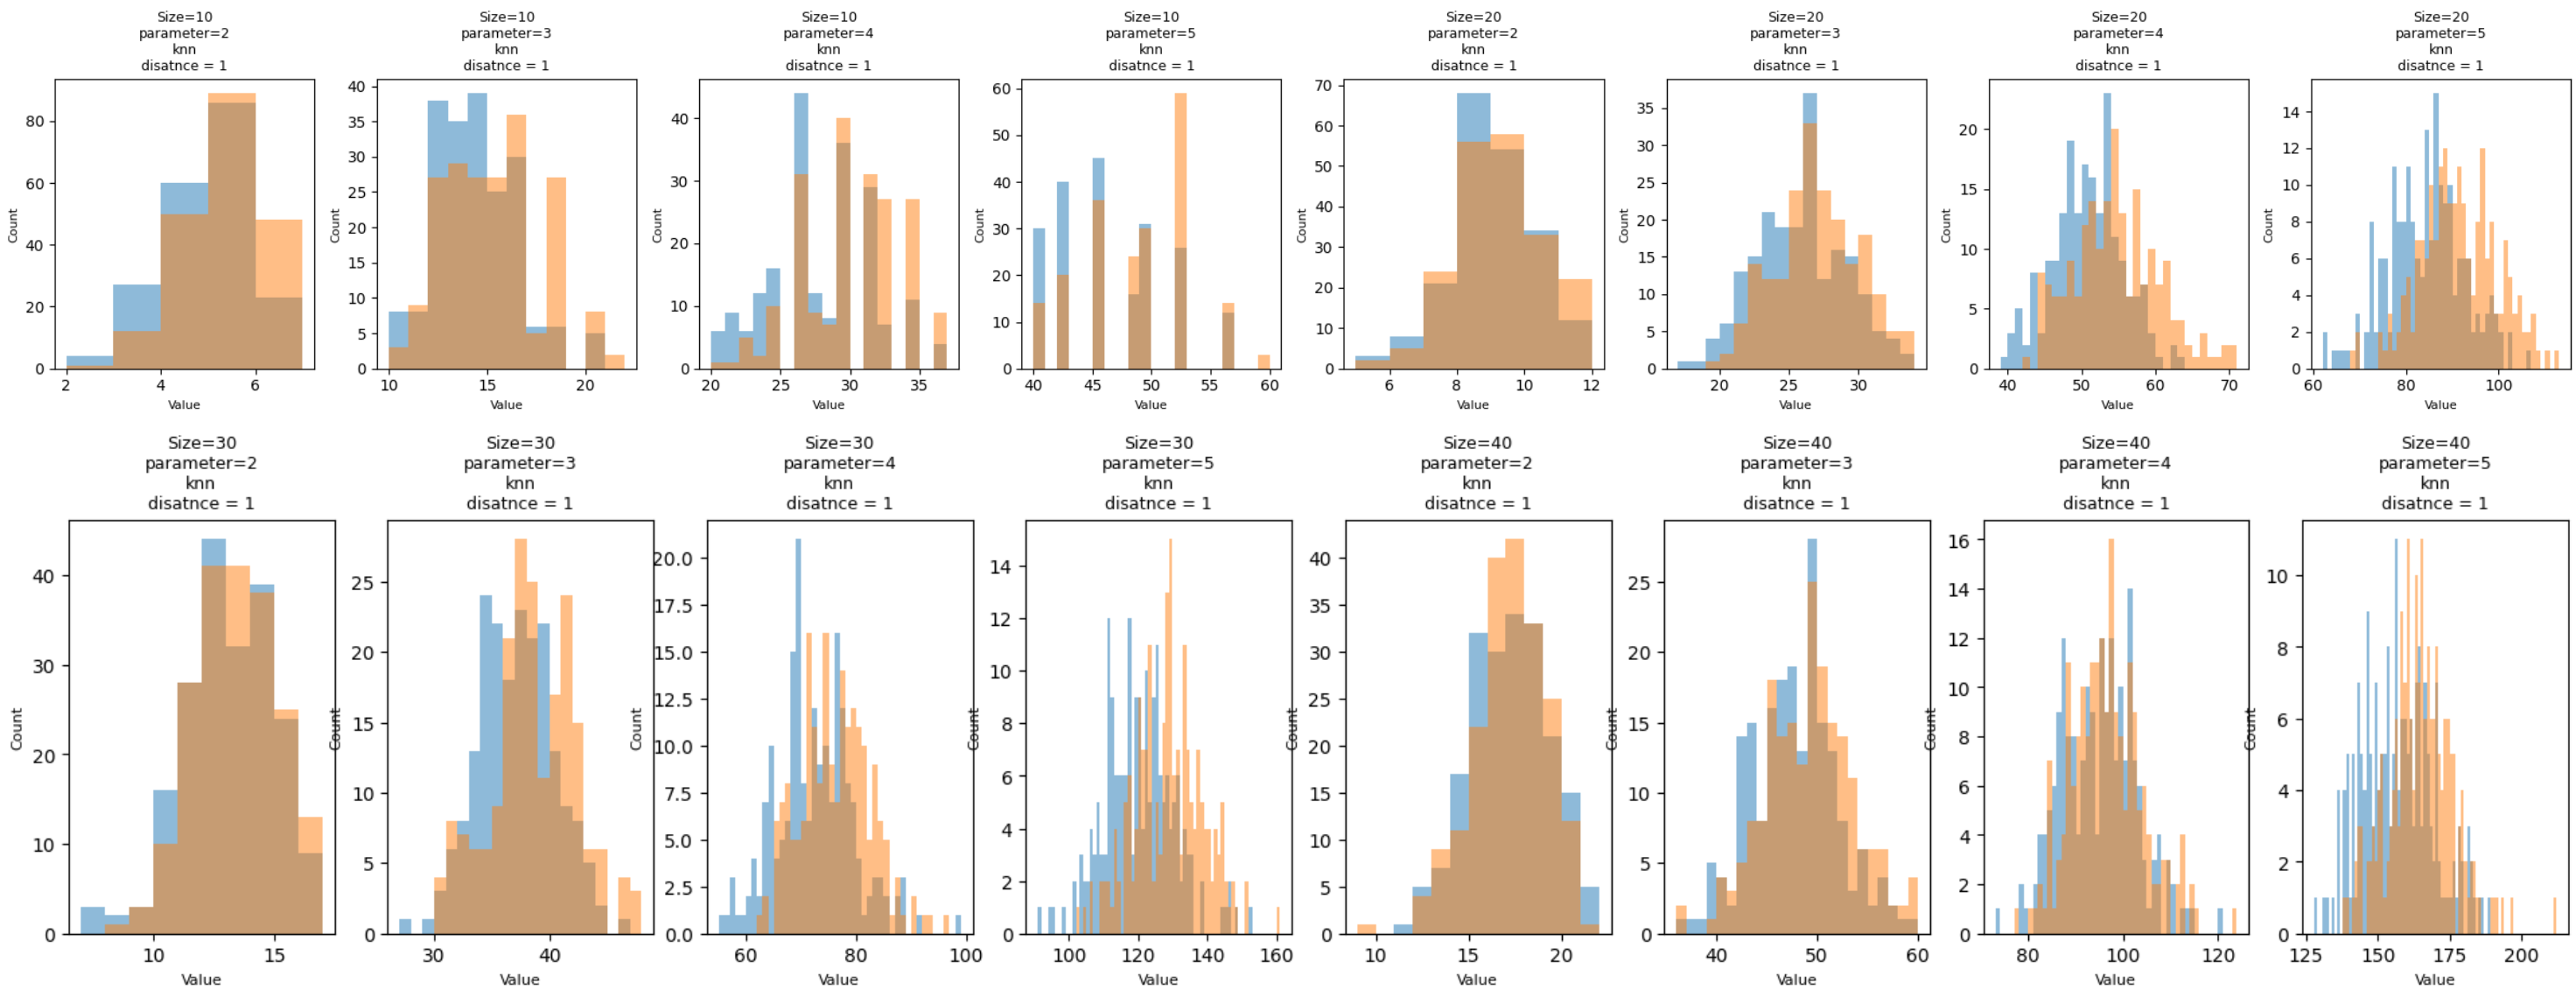
\includegraphics[width=1\textwidth]{Part-I-Ivanova/2_1_hist.png}

\noindent\textbf{Вывод:} При любом размере выборки количество треугольников не выглядит хорошей характеристикой, потому что графики практически идентичны. Лучшее, что можно получить, при количестве вершин 40 и количестве соседей в графе - 5 (правый нижний график)
\\
\noindent\textbf{Графики для дистанционного графа}
\\
\hspace*{-0.5cm}
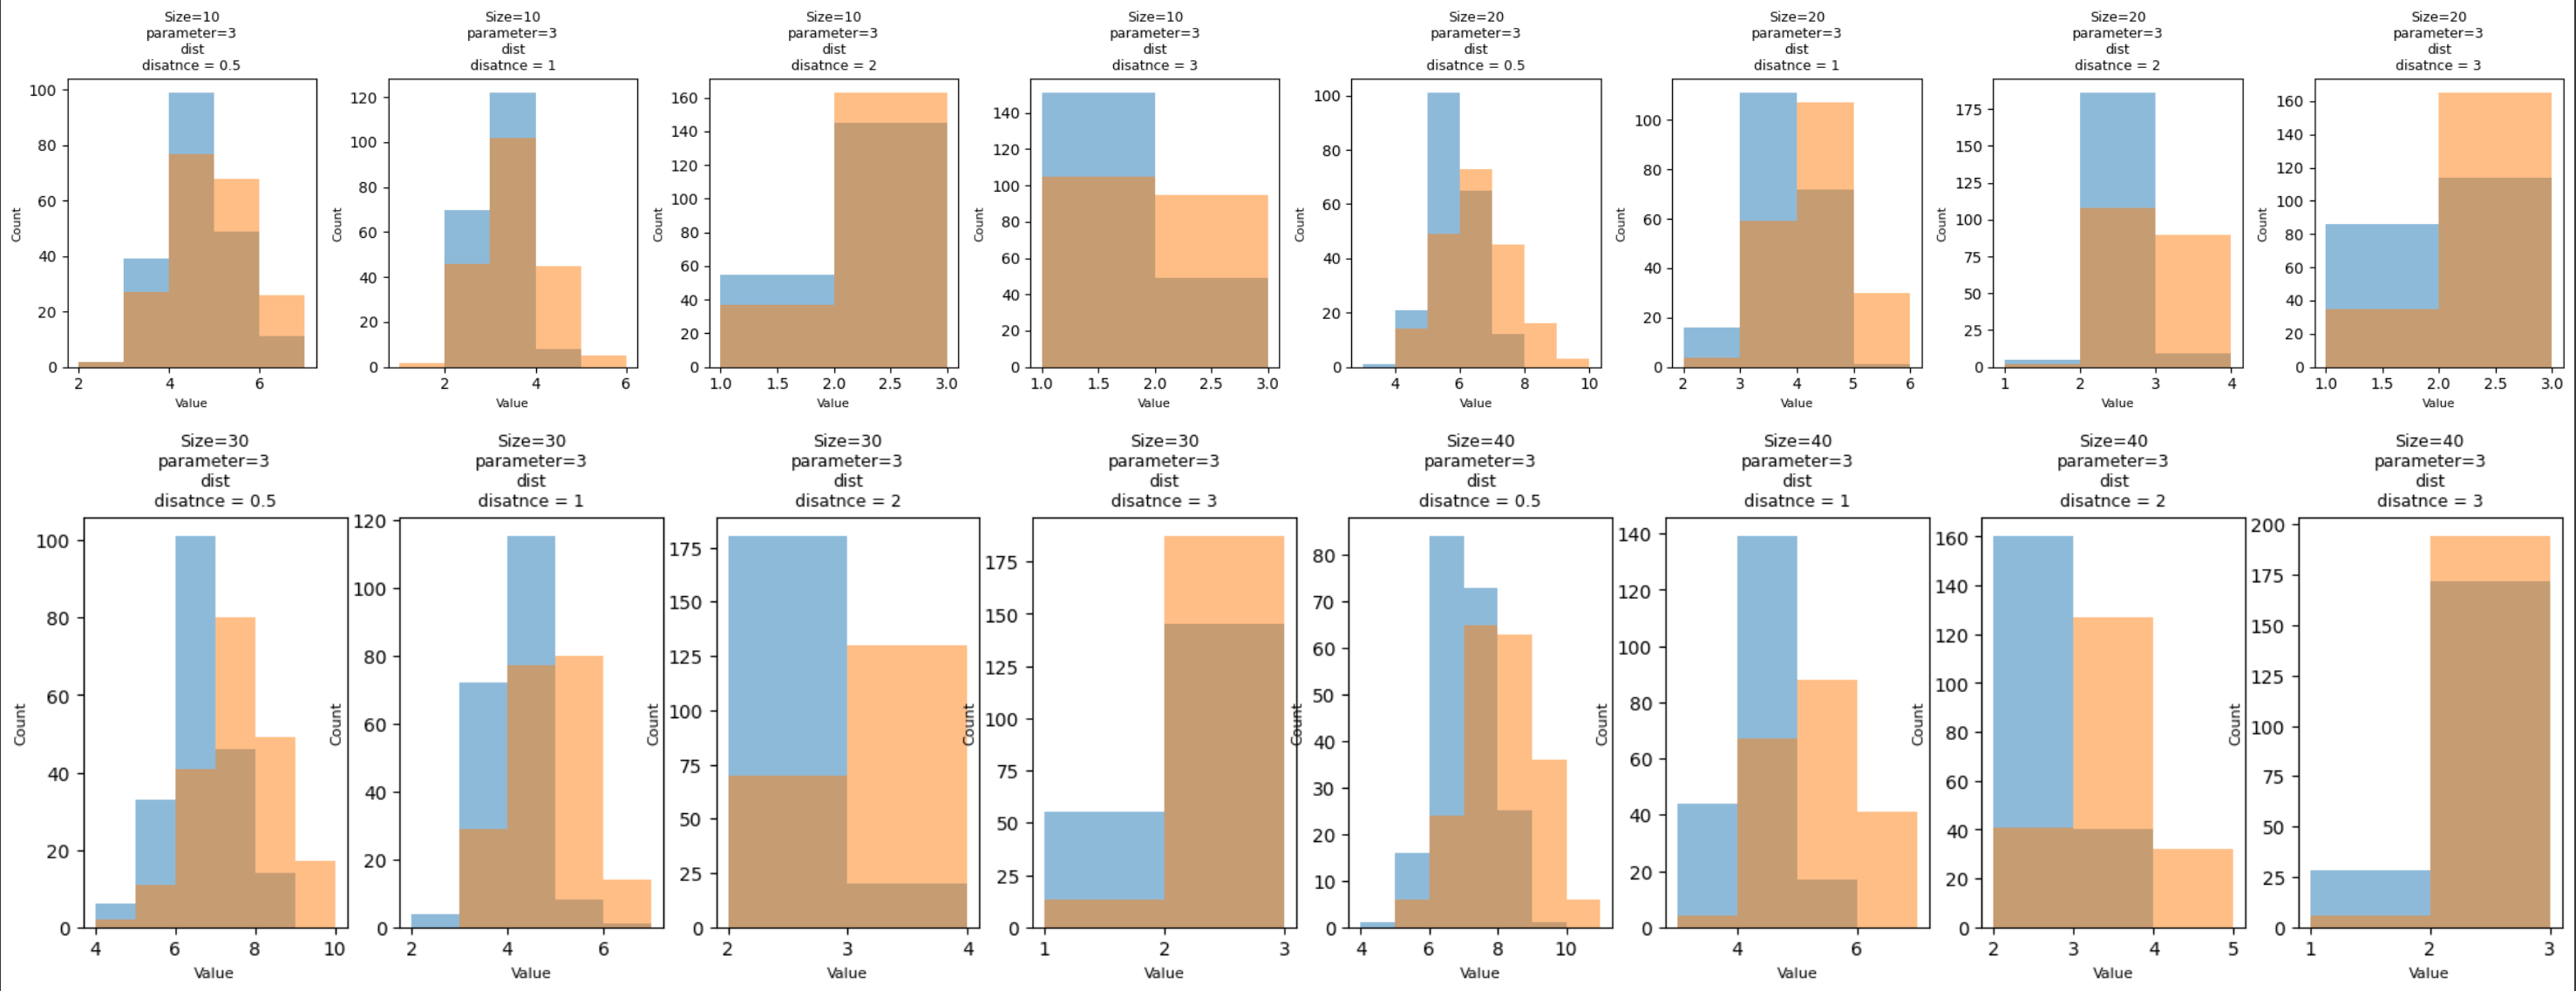
\includegraphics[width=1\textwidth]{Part-I-Ivanova/2_2_hist.png}\\ 


\noindent \textbf{Вывод:} Максимальное независимое множество, с точки зрения задачи классификации, для данных распределений является признаком получше, например для 40 вершин и дистанции 2, распределения уже неплохо различимы, на основе этой характеристики и будем строить критическое множество. 

\newpage

\subsection*{2.3 Построение критического множества и оценка мощности критерия}

\noindent Построение критического множества $\mathcal{A}$ происходит следующим образом:\\
1. Генерируем большое количество графов, с фиксированными параметрами и считаем для каждого из них характеристику.\\
2. Считаем $95\%$ перцентиль = $A_{crit}$ - это будет крайнее значение множества $\mathcal{A}$ \\
3. Теперь, если значение характеристики графа $\leq A_{crit}$, то принимаем гипотезу $H_0$, иначе отвергаем\\

\vspace{5pt}
\noindent \textbf{Минаков Д.Д.}\\\\
\noindentДля распределений \qquad\qquad Weibull$(\ \frac{1}{2}, \frac{1}{\sqrt{10}}) \qquad\qquad \Gamma(\ \frac{1}{2}, \frac{1}{\sqrt2}) $\\\\
и \textbf{Distance} графа, по характеристике \textbf{кликовое число} построим критическое множество $A$.\\

\noindent$H_0 - $ гамма распределение, $H_1 - $ распределение Вейбулла.

\noindentПолучим:\\
Критическое значение $A_{crit} = 46$.\\
Мощность критерия = $0.31120000$\\
Ошибка 1 рода : $0.02190000$\\
    
\vspace{10pt}
\noindent \textbf{Иванова А.А.}\\\\

\noindent \textbf{Итоги Ивановой А.А.}

\begin{table}[h]
\centering
\begin{tabular}{lcc}
\toprule
\textbf{Размер выборки} & \textbf{Ошибка I рода ($\alpha$)} & \textbf{Мощность критерия} \\
\midrule
N = 25   & 0.21 & 0.7086 \\
N = 100  & 0.06 & 0.9153 \\
N = 500  & 0.00 & 1.0000 \\
\bottomrule
\end{tabular}
\label{tab:power_analysis}
\end{table}

\noindent \textbf{Общий анализ:}\\
На 500 вершинах можно точно отличить распределения, потому что у них сильно отличаются характеристики, но это достаточно долго, поэтому лучше выбрать 100 вершин, ошибка первого рода 0.06 и 0.03 соответственно, мощность 0.92 и 0.97 соответственно, но при этом обсчет 10к графов займет всего 10 минут\\

\noindent \textbf{Общий вывод:}\\
Классификатор имеет высокую мощность и маленькую ошибку первого рода на 3000 вычислениях, что делает его отличным статистическим критерием.
\noindent
\newpage

\section*{3. Part-II}
\subsection*{3.1 Применяем классификационные алгоритмы (Минаков Д.Д.)}

Выберем 3 модели - линейная, логистическая и ridge регрессии, обучим на них классификатор и сравним качество

\begin{table}[h]
    \centering
    \label{tab:results}
    \begin{tabular}{cccccc}
    \toprule
    N & Модель & Precision & Accuracy & Recall \\
    \midrule
    \multirow{3}{*}{25} 
        & Logistic & 0.8071 & 0.8037 & 0.7980 \\
        & Linear & 0.8426 & 0.8077 & 0.7567 \\
        & Ridge & 0.8426 & 0.8077 & 0.7567 \\
    \hline
    \multirow{3}{*}{100} 
        & Logistic & 0.9700 & 0.9693 & 0.9687 \\
        & Linear & 0.9907 & 0.9597 & 0.9280 \\
        & Ridge & 0.9907 & 0.9597 & 0.9280 \\
    \hline
    \multirow{3}{*}{500} 
        & Logistic & 1.0000 & 0.9993 & 0.9987 \\
        & Linear & 1.0000 & 0.9993 & 0.9987 \\
        & Ridge & 1.0000 & 0.9993 & 0.9987 \\
    \bottomrule
    \end{tabular}
\end{table}

Все линейные модели дают очень близкий результат, поэтому зафиксируем в качестве модели обычную \textbf{логистическую регрессию}\\

\textbf{Проведем кроссвалидацию для оценки дисперсии метрик}\\

\hspace*{-1cm}
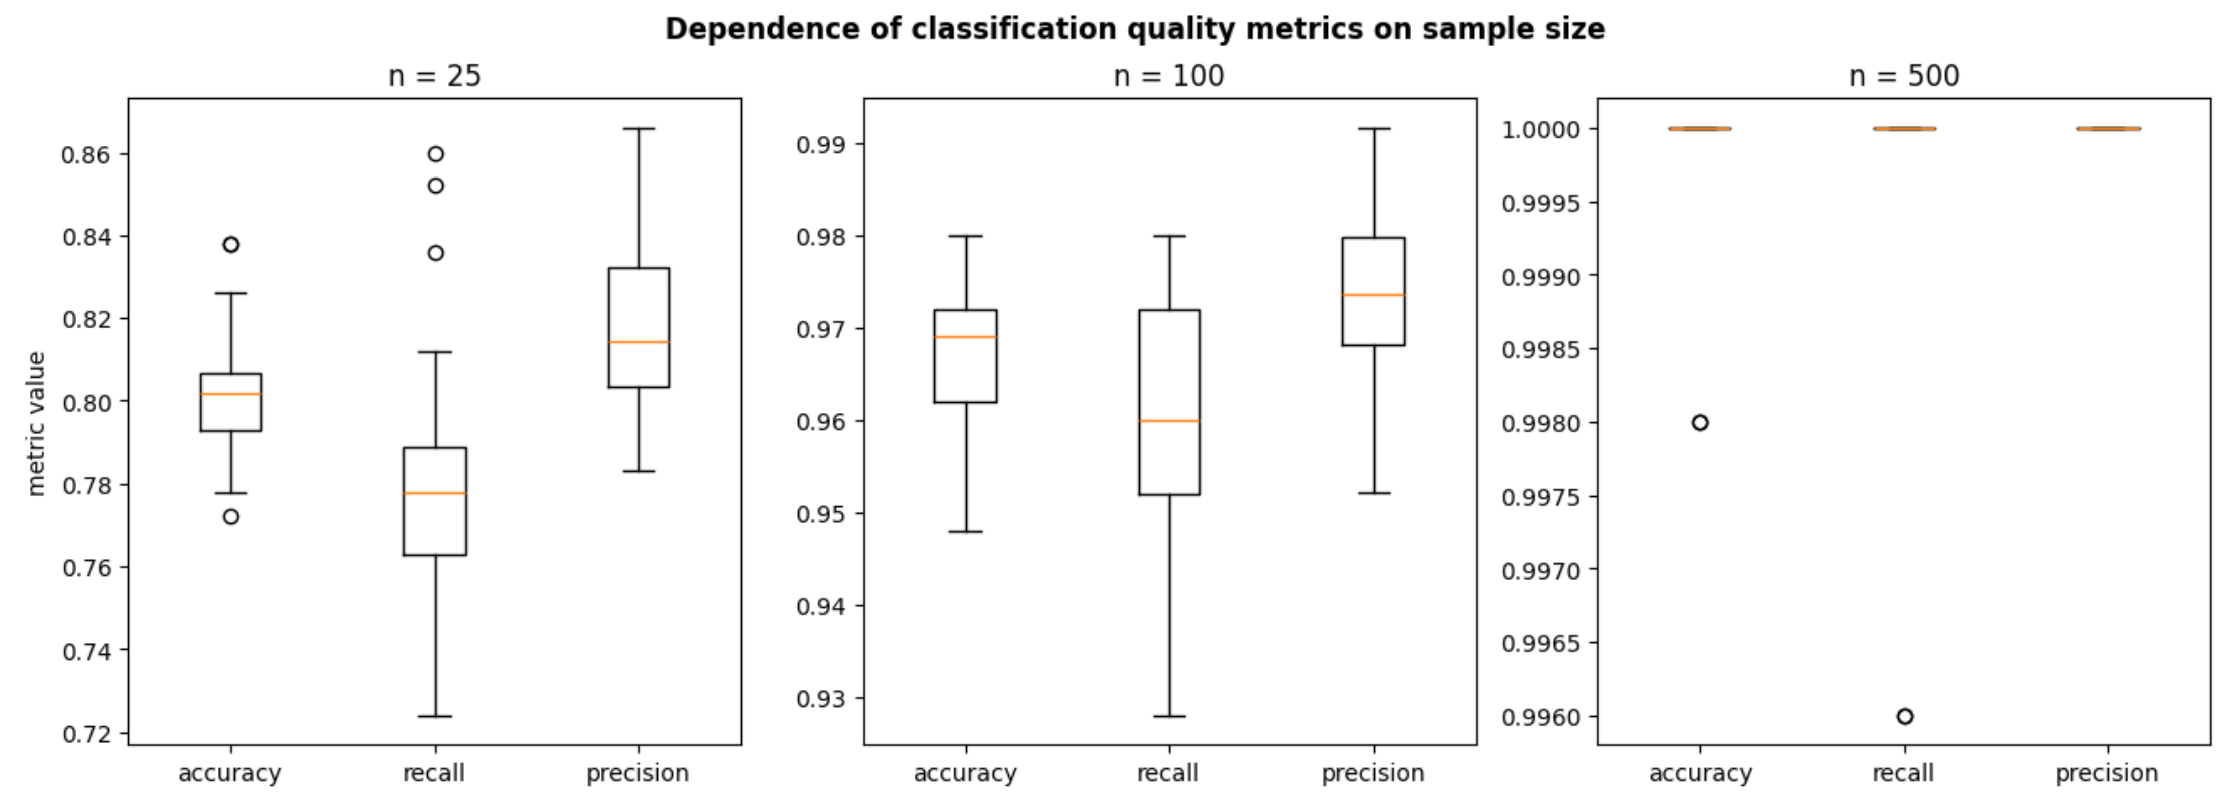
\includegraphics[width=1\textwidth]{Part-II_student-2/dependence metrics on sample size}\\ 

\textbf{Занесем данные в таблицу}\\

\begin{table}[h]
    \centering
    \begin{tabular}{lccc}
    \toprule
    \textbf{Размер выборки} & \textbf{Метрика} & \textbf{Среднее} & \textbf{Дисперсия} \\
    \midrule
    \multirow{3}{*}{N=25} 
     & Accuracy  & 0.80  & 0.000271 \\
     & Recall    & 0.78  & 0.001231 \\
     & Precision & 0.81  & 0.000460 \\
    \midrule
    \multirow{3}{*}{N=100}
     & Accuracy  & 0.97  & $6.384 \times 10^{-5}$ \\
     & Recall    & 0.96  & 0.000166 \\
     & Precision & 0.97  & $9.624 \times 10^{-5}$ \\
    \midrule
    \multirow{3}{*}{N=500}
     & Accuracy  & 0.999 & $3.6 \times 10^{-7}$ \\
     & Recall    & 0.999 & $1.44 \times 10^{-6}$ \\
     & Precision & 0.99  & 0.0 \\
    \bottomrule
    \end{tabular}
\end{table}

\noindent\textbf{Выводы:}
\begin{itemize}
    \item Увеличение выборки снижает дисперсию экспоненциально

    \item \textbf{Стабильность метрик:}
        \begin{itemize}
            \item Precision демонстрирует самую низкую дисперсию на всех выборках
            \item Recall наиболее чувствителен к размеру выборки

        \end{itemize}
    
    \item \textbf{Оптимальный размер:} Для данной задачи выборка размером n=100 уже обеспечивает отличные результаты, а дальнейшее увеличение (n=500) лишь незначительно улучшает метрики и их стабильность.
\end{itemize}

\restoregeometry

\subsection*{3.1 Применяем классификационные алгоритмы (Иванова А.А.)}
Посмотрим на поведение характеристик при фиксированных параметрах построения графов для распределения Лапласа и косого нормального, с варьирующимися параметрами распределений. Ниже графики, на которых перебираются различные параметры $\alpha_{laplace}, \beta_{laplace}, \alpha_{skew}$ при фиксированных параметрах графа:
\begin{itemize}
    \item Размер графа =  40
    \item K в KNN = 3
    \item dist в Distance = 1
    \item характеристика для KNN графа - число треугольников (на этой странице)
    \item характеристика для Dist графа - максимальное независимое множество
\end{itemize}
\\

\hspace*{-1cm}
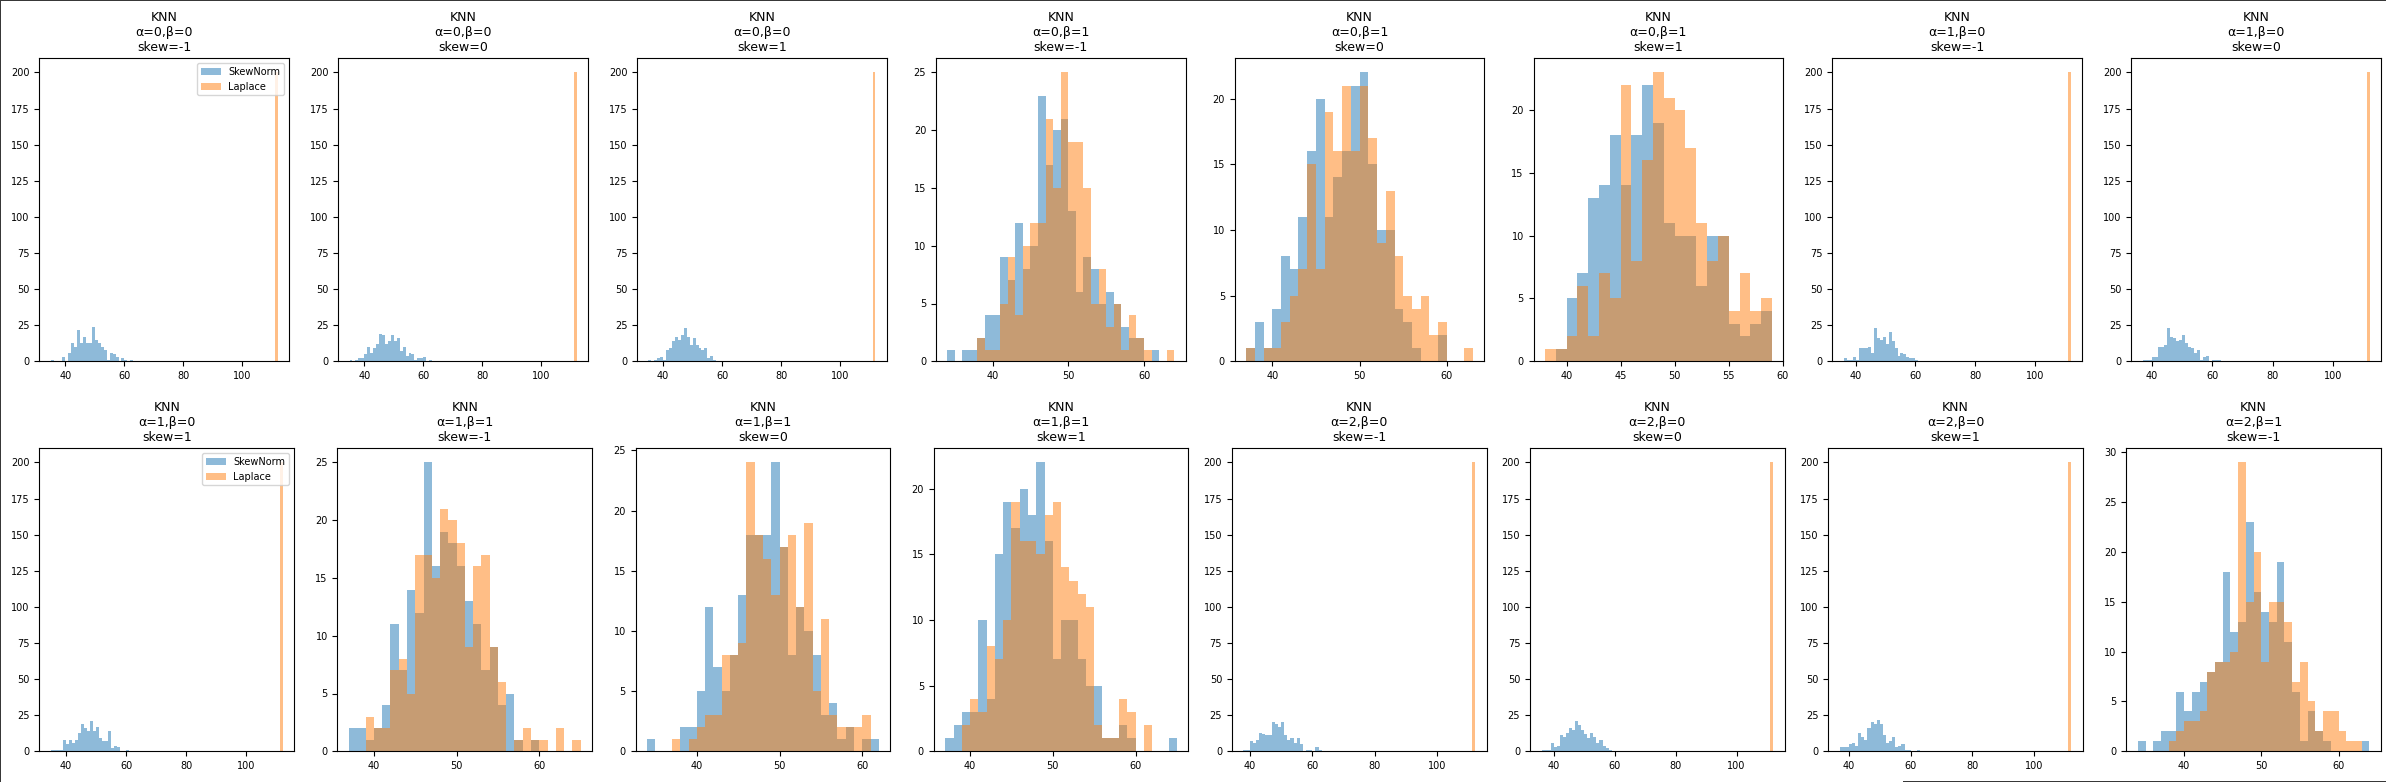
\includegraphics[width=1\textwidth]{Part-I-Ivanova/1_hist.png}\\ 
\hspace*{-0.5cm}
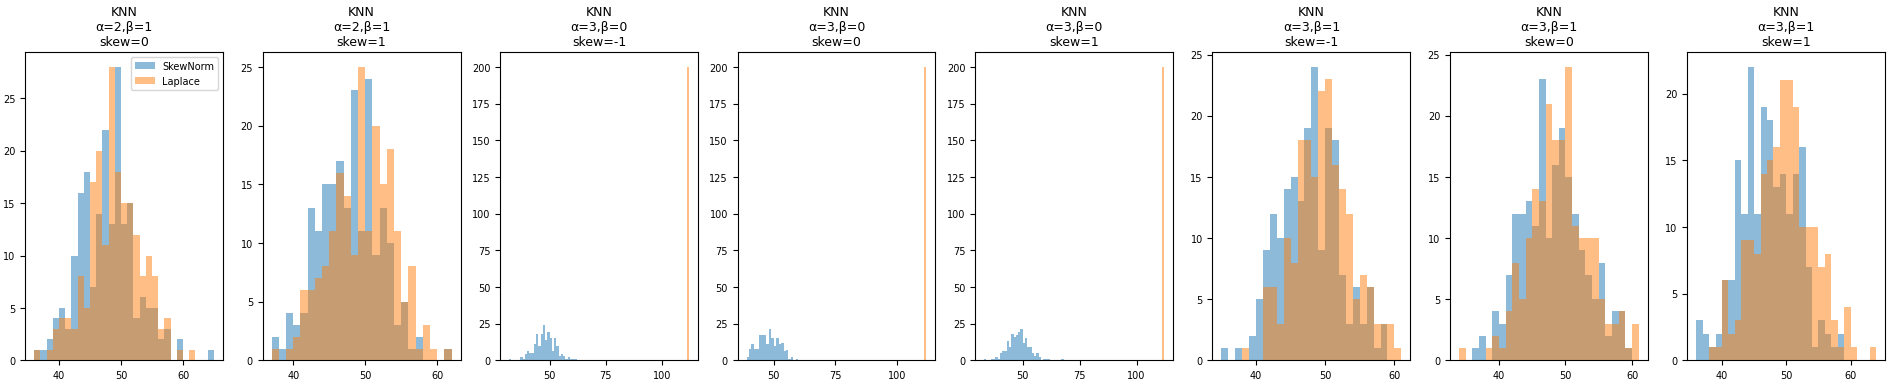
\includegraphics[width=1\textwidth]{Part-I-Ivanova/4_hist.png}\\ 
\textbf{Вывод:} в зависимости от параметров распределений характеристика 'Количество треугольников' KNN графа может быть \textbf{очень хорошим} признаком классификации при хороших параметрах распределений, а при некоторых графики практически идентичны, распределения трудно отличимы.
\newpage
\noindent\textbf{Далее графики для дистанционного графа :} \\\\


\hspace*{-1cm}
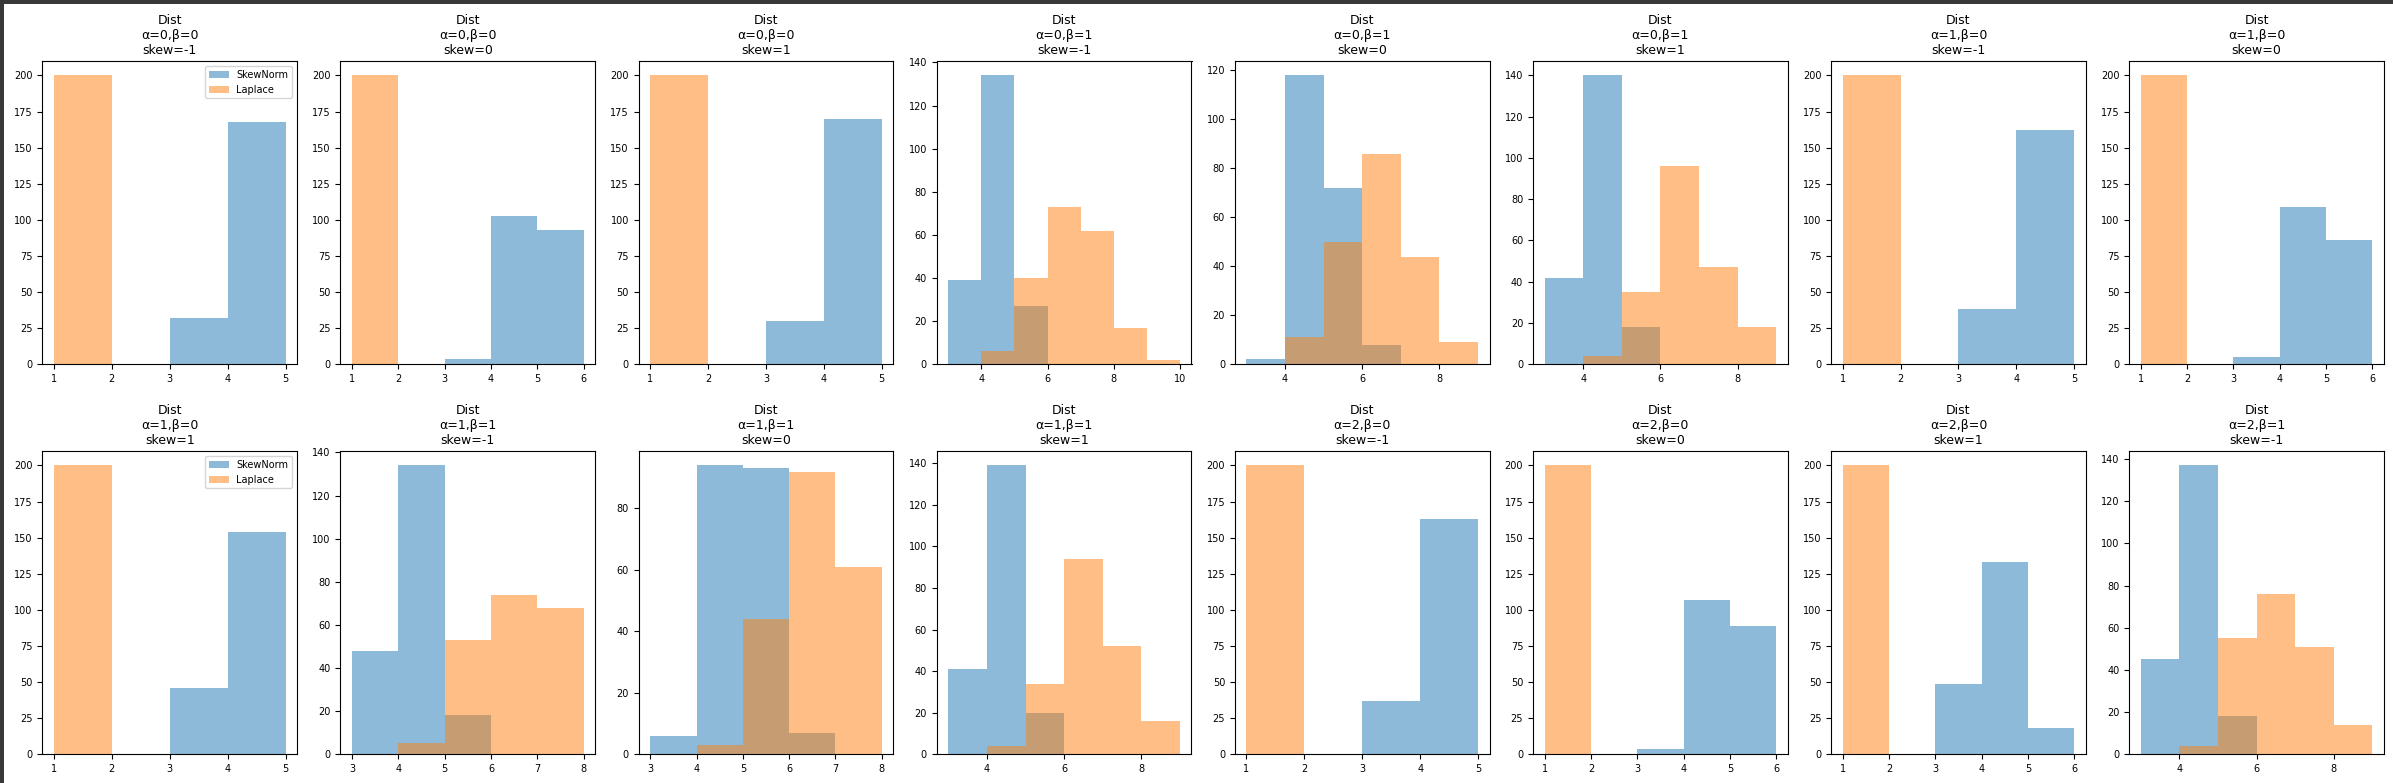
\includegraphics[width=1\textwidth]{Part-I-Ivanova/2_hist.png}
\\
\hspace*{-0.5cm}
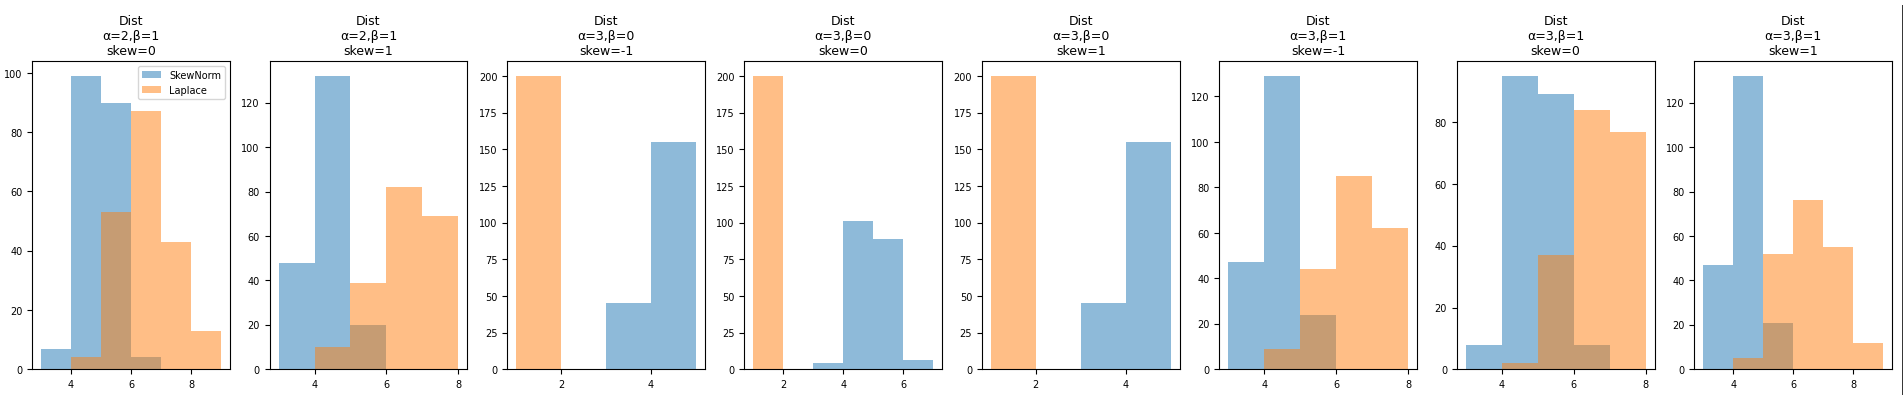
\includegraphics[width=1\textwidth]{Part-I-Ivanova/3_hist.png}\\ 


\noindent\textbf{Вывод:} в целом характеристика 'Размер максимального независимого множества' неплохая характеристика, при некоторых параметрах она лучше разделяет распределения, в некоторых хуже, но в целом всегда неплохо.


\subsection*{3.2 Важность характеристик, как признаков классификации (Минаков Д.Д.)}

Теперь посмотрим на поведение характеристик в зависимости от параметров построения графов, при фиксированных распределениях
\begin{equation*}
    \text{Weibull}(\ \frac{1}{2}, \frac{1}{\sqrt{10}}) \qquad\qquad \Gamma(\ \frac{1}{2}, \frac{1}{\sqrt2})
\end{equation*}

\hspace*{-1cm}
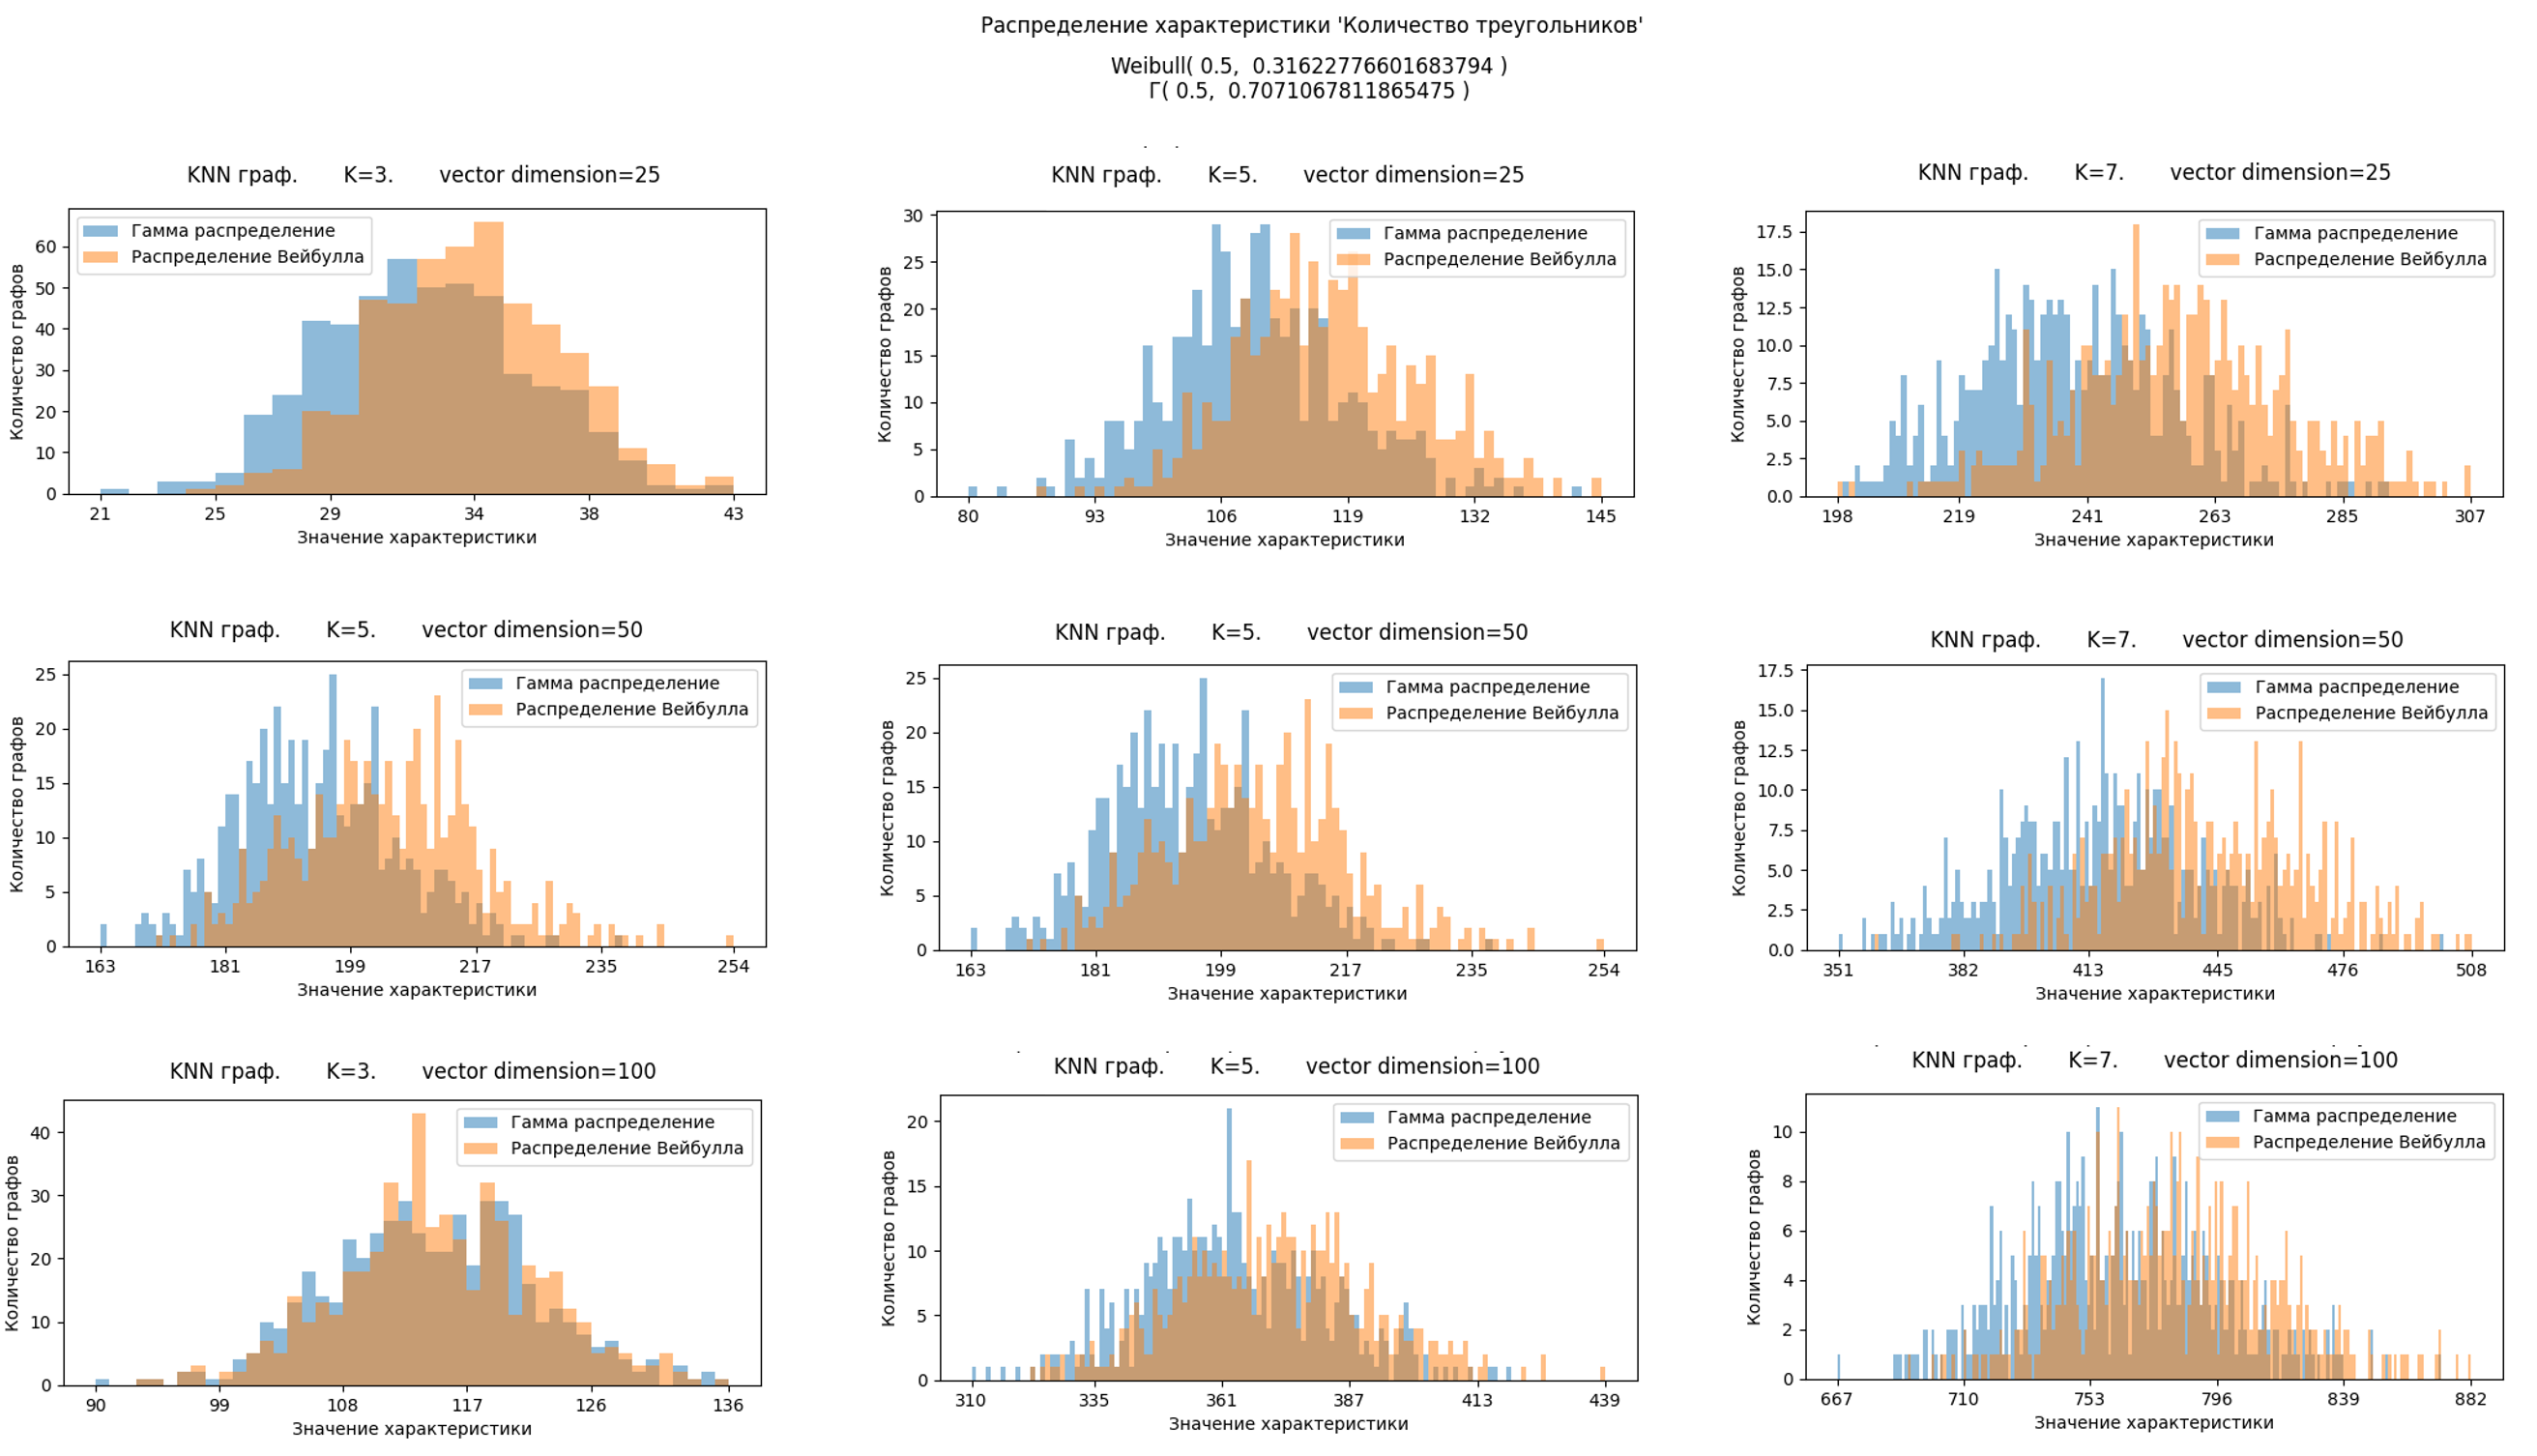
\includegraphics[width=1\textwidth]{Part-I_student-2/point 2_histogram_KNN.png}\\ 

\textbf{Вывод:} при большом размере выборки, количество треугольников выглядит как не самая удачная характеристика для классификации, однако, при относительно небольшой выборке ($\leq 50$), эта характеристика может оказаться неплохим второстепенным признаком.\\ 

\hspace*{-1cm}
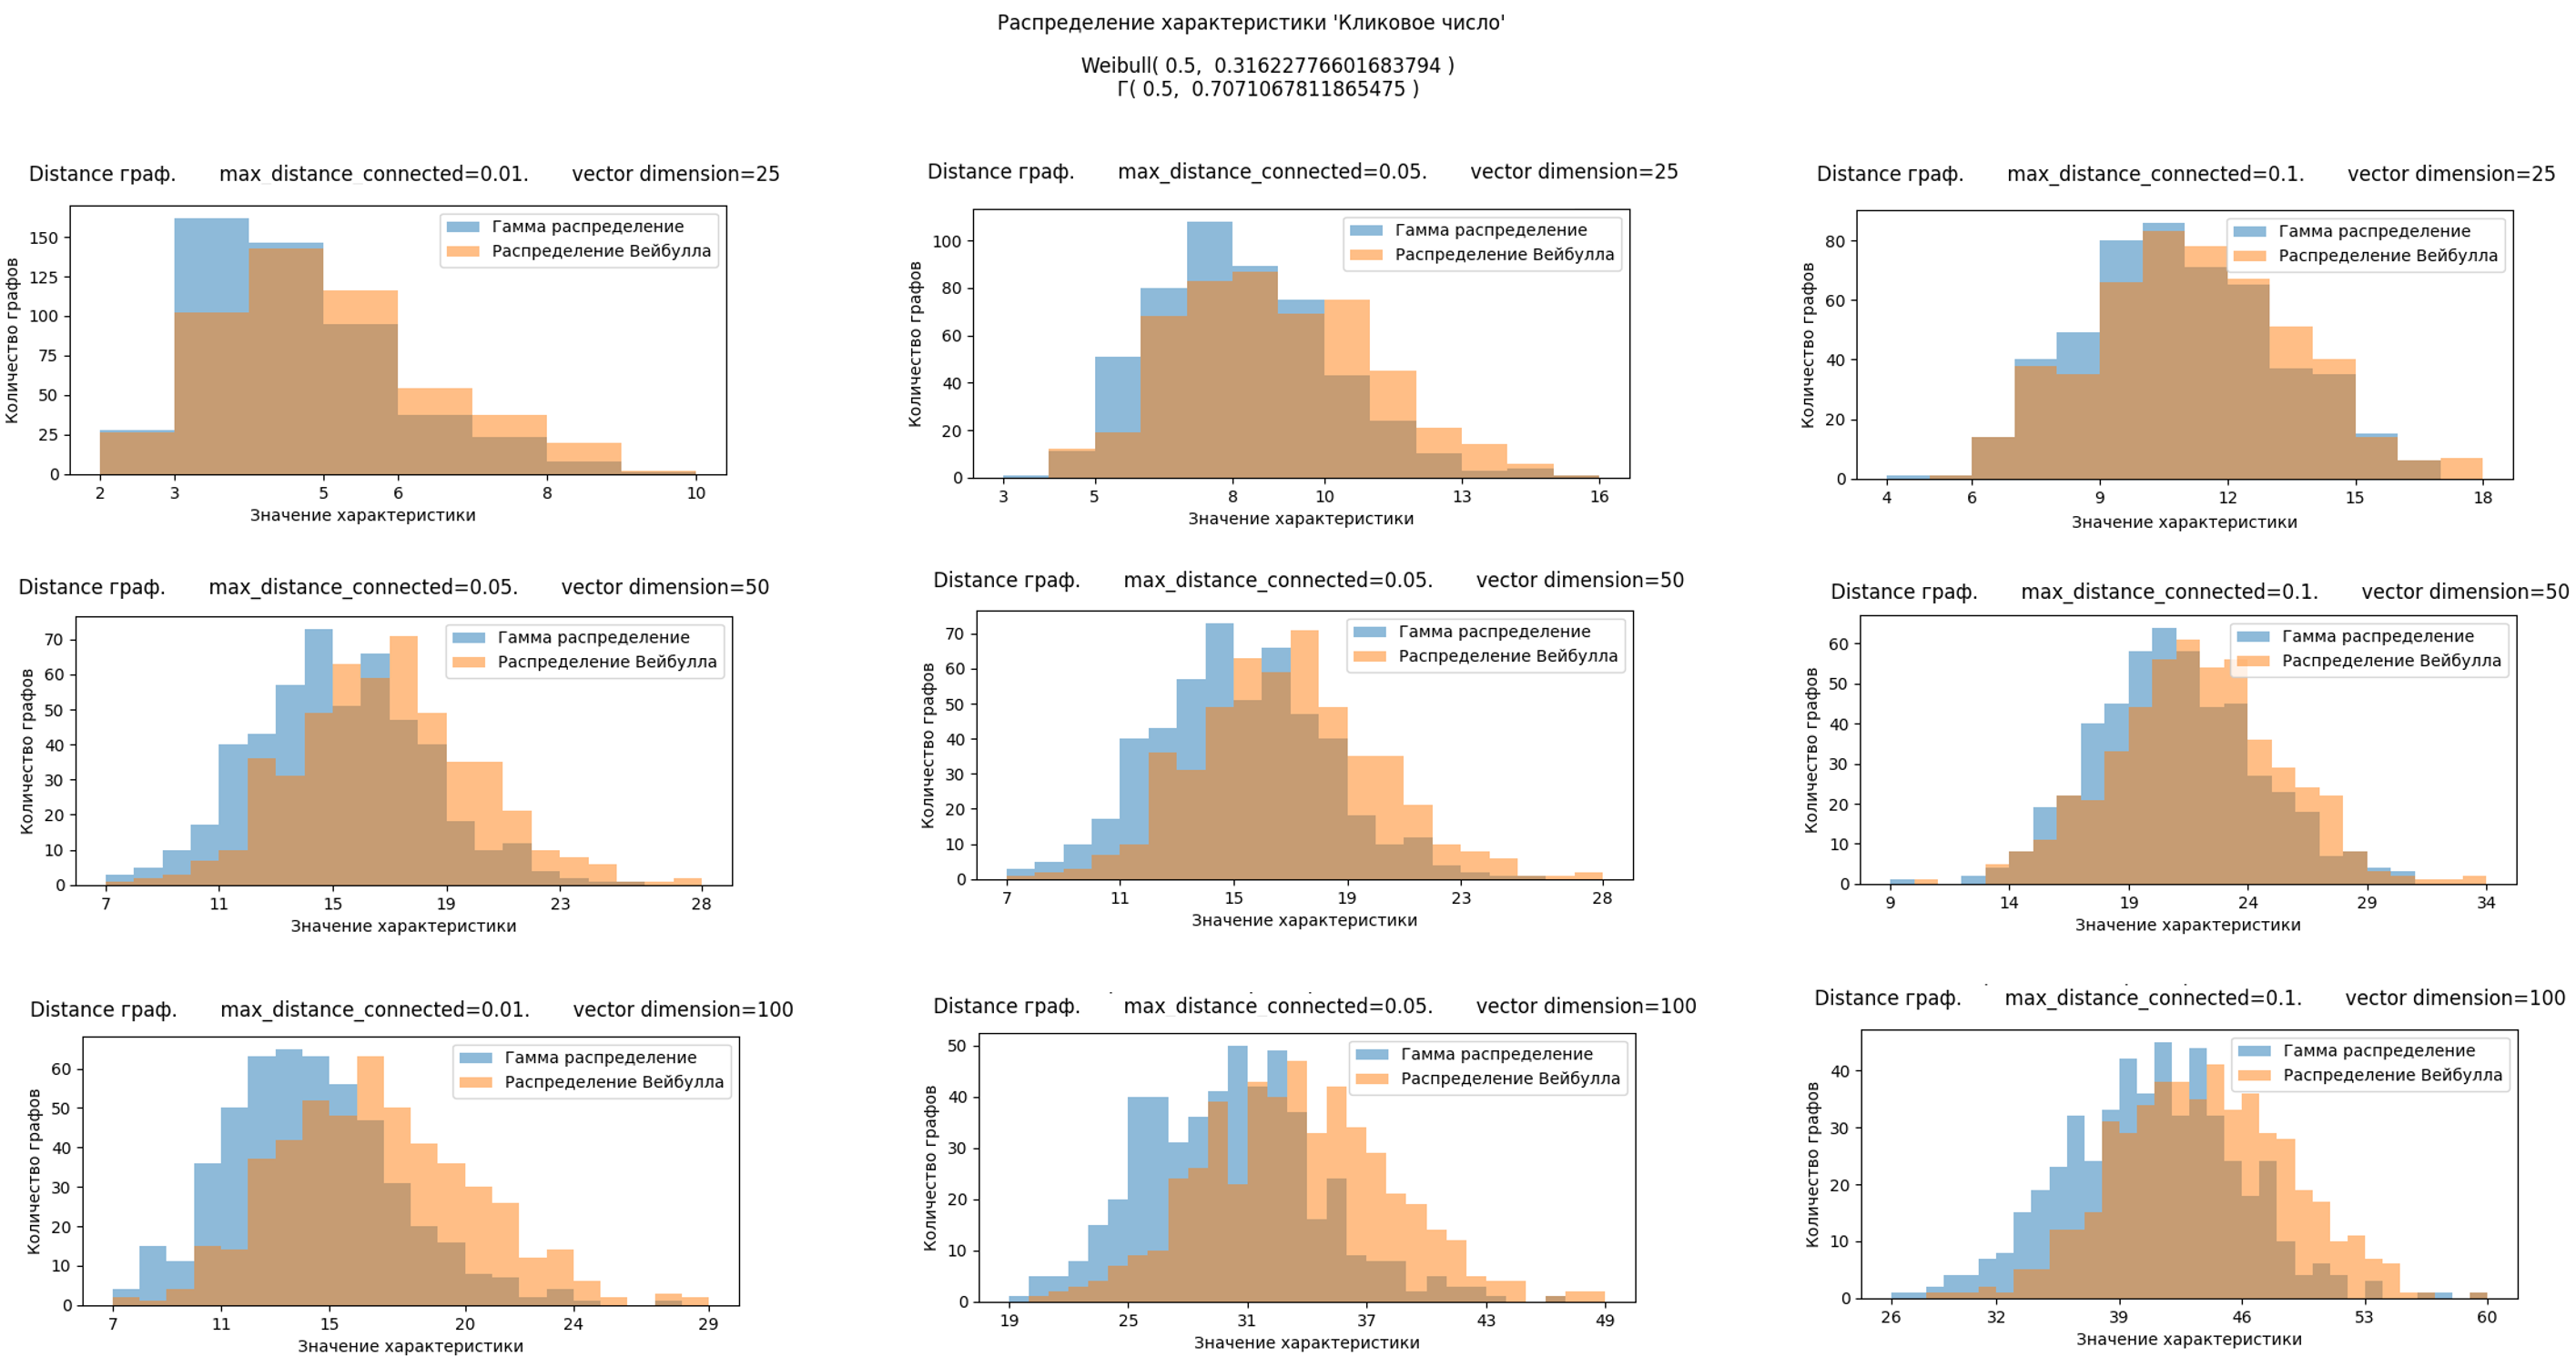
\includegraphics[width=1\textwidth]{Part-I_student-2/point 2_histogram_Dist.png}\\ 

\textbf{Вывод:} кликовое число, с точки зрения задачи классификации, для данных распределений является посредственным признаком, независимо от размера выборки и расстояния связи. Убедиться в этом  еще раз мы сможем в \textbf{Part-II}. 
\newpage
\subsection*{3.2 Важность характеристик, как признаков классификации (Иванова А.А.)}

Теперь посмотрим на поведение характеристик в зависимости от параметров построения графов, при фиксированных распределениях
\\
\begin{equation*}
    \text{Laplace}(\ 0, \frac{1}{\sqrt{2}}) \qquad\qquad Skewnormal (1)
\end{equation*}
\textbf{Графики для KNN графа :}


\hspace*{-1cm}
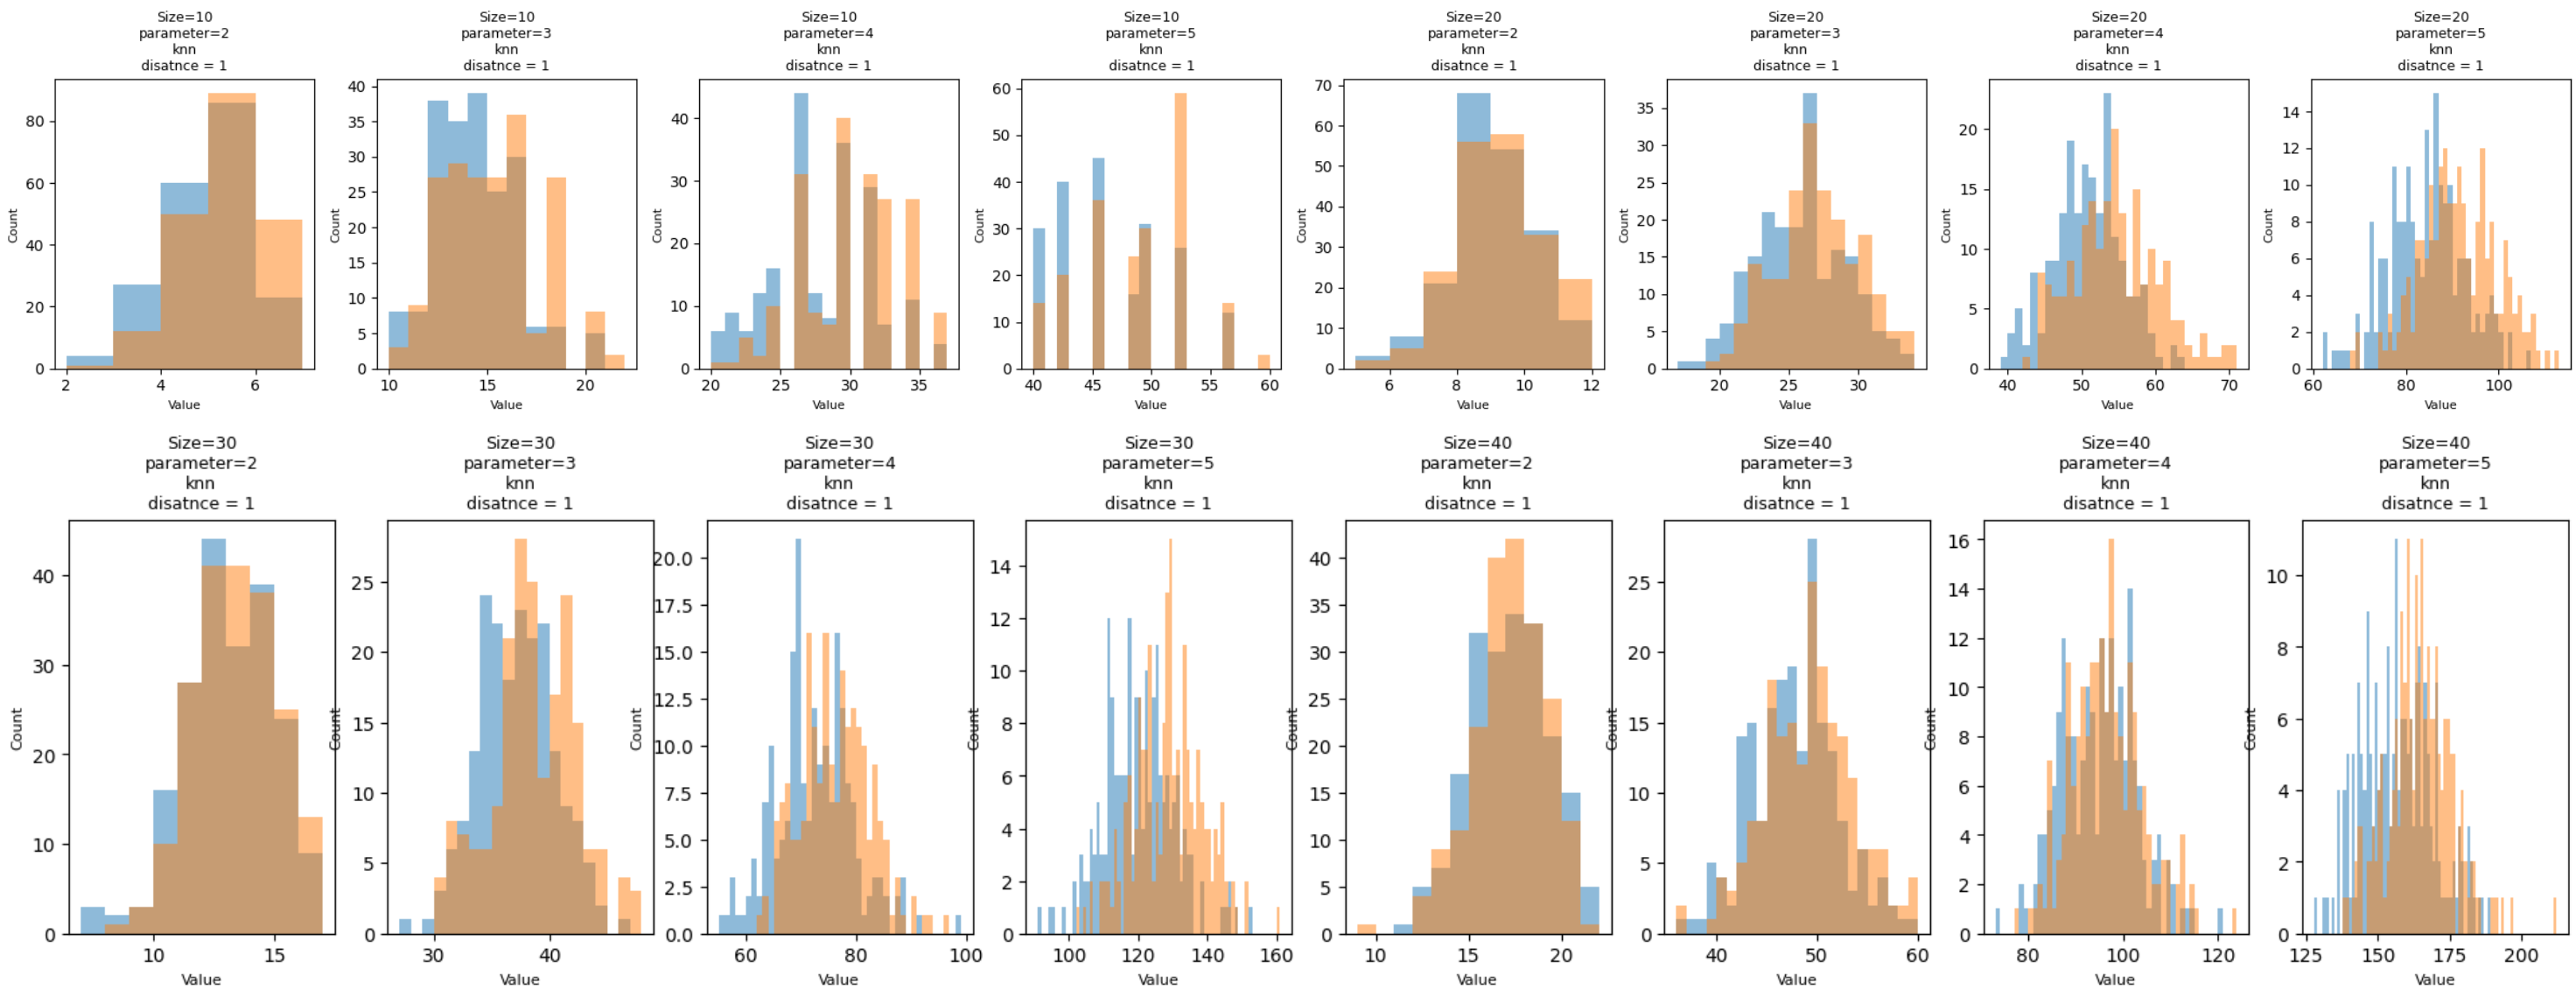
\includegraphics[width=1\textwidth]{Part-I-Ivanova/2_1_hist.png}

\noindent\textbf{Вывод:} При любом размере выборки количество треугольников не выглядит хорошей характеристикой, потому что графики практически идентичны. Лучшее, что можно получить, при количестве вершин 40 и количестве соседей в графе - 5 (правый нижний график)
\\
\noindent\textbf{Графики для дистанционного графа}
\\
\hspace*{-0.5cm}
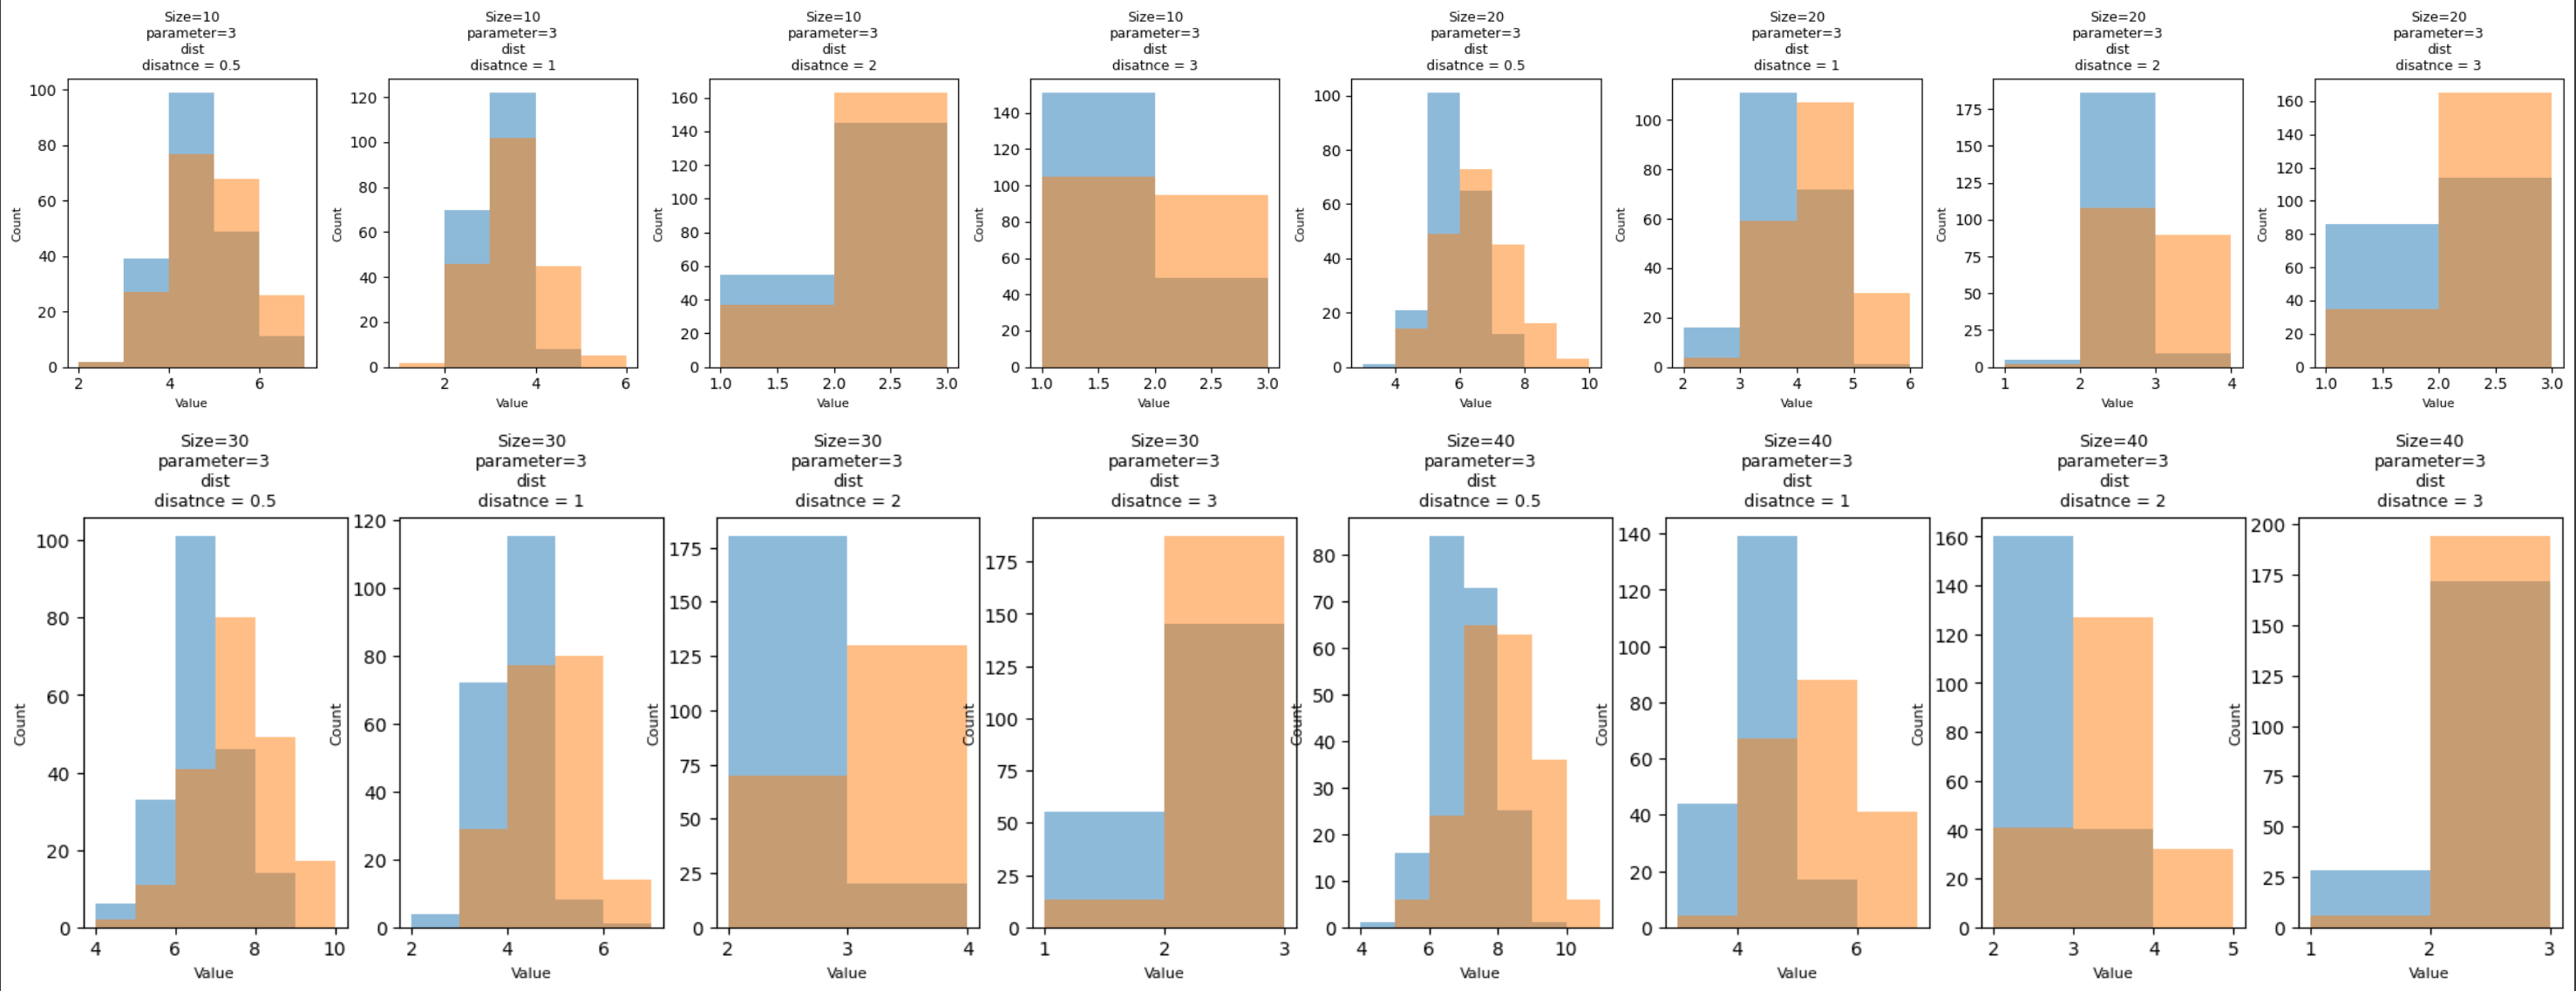
\includegraphics[width=1\textwidth]{Part-I-Ivanova/2_2_hist.png}\\ 


\noindent \textbf{Вывод:} Максимальное независимое множество, с точки зрения задачи классификации, для данных распределений является признаком получше, например для 40 вершин и дистанции 2, распределения уже неплохо различимы, на основе этой характеристики и будем строить критическое множество. 

\newpage

\subsection*{3.3 Выводы о вероятности ошибки первого рода и мощности модели как критерия}
\noindentДля распределений \qquad\qquad Weibull$(\ \frac{1}{2}, \frac{1}{\sqrt{10}}) \qquad\qquad \Gamma(\ \frac{1}{2}, \frac{1}{\sqrt2}) $\\\\
и \textbf{Distance} графа, по характеристике \textbf{кликовое число} построим критическое множество $A$.\\

\noindent$H_0 - $ гамма распределение, $H_1 - $ распределение Вейбулла.

\noindentПолучим:\\
Критическое значение $A_{crit} = 46$.\\
Мощность критерия = $0.31120000$\\
Ошибка 1 рода : $0.02190000$\\

\noindent \textbf{Итоги Ивановой А.А.}

\begin{table}[h]
\centering
\begin{tabular}{lcc}
\toprule
\textbf{Размер выборки} & \textbf{Ошибка I рода ($\alpha$)} & \textbf{Мощность критерия} \\
\midrule
N = 25   & 0.21 & 0.7086 \\
N = 100  & 0.06 & 0.9153 \\
N = 500  & 0.00 & 1.0000 \\
\bottomrule
\end{tabular}
\label{tab:power_analysis}
\end{table}

\noindent \textbf{Общий анализ:}\\
На 500 вершинах можно точно отличить распределения, потому что у них сильно отличаются характеристики, но это достаточно долго, поэтому лучше выбрать 100 вершин, ошибка первого рода 0.06 и 0.03 соответственно, мощность 0.92 и 0.97 соответственно, но при этом обсчет 10к графов займет всего 10 минут\\

\noindent \textbf{Общий вывод:}\\
Классификатор имеет высокую мощность и маленькую ошибку первого рода на 3000 вычислениях, что делает его отличным статистическим критерием.
\noindent
        
\end{document}